\documentclass[mstat,12pt]{unswthesis}

\usepackage{color}
\usepackage{fancyvrb}
\newcommand{\VerbBar}{|}
\newcommand{\VERB}{\Verb[commandchars=\\\{\}]}
\DefineVerbatimEnvironment{Highlighting}{Verbatim}{commandchars=\\\{\}}
% Add ',fontsize=\small' for more characters per line
\usepackage{framed}
\definecolor{shadecolor}{RGB}{248,248,248}
\newenvironment{Shaded}{\begin{snugshade}}{\end{snugshade}}
\newcommand{\AlertTok}[1]{\textcolor[rgb]{0.94,0.16,0.16}{#1}}
\newcommand{\AnnotationTok}[1]{\textcolor[rgb]{0.56,0.35,0.01}{\textbf{\textit{#1}}}}
\newcommand{\AttributeTok}[1]{\textcolor[rgb]{0.13,0.29,0.53}{#1}}
\newcommand{\BaseNTok}[1]{\textcolor[rgb]{0.00,0.00,0.81}{#1}}
\newcommand{\BuiltInTok}[1]{#1}
\newcommand{\CharTok}[1]{\textcolor[rgb]{0.31,0.60,0.02}{#1}}
\newcommand{\CommentTok}[1]{\textcolor[rgb]{0.56,0.35,0.01}{\textit{#1}}}
\newcommand{\CommentVarTok}[1]{\textcolor[rgb]{0.56,0.35,0.01}{\textbf{\textit{#1}}}}
\newcommand{\ConstantTok}[1]{\textcolor[rgb]{0.56,0.35,0.01}{#1}}
\newcommand{\ControlFlowTok}[1]{\textcolor[rgb]{0.13,0.29,0.53}{\textbf{#1}}}
\newcommand{\DataTypeTok}[1]{\textcolor[rgb]{0.13,0.29,0.53}{#1}}
\newcommand{\DecValTok}[1]{\textcolor[rgb]{0.00,0.00,0.81}{#1}}
\newcommand{\DocumentationTok}[1]{\textcolor[rgb]{0.56,0.35,0.01}{\textbf{\textit{#1}}}}
\newcommand{\ErrorTok}[1]{\textcolor[rgb]{0.64,0.00,0.00}{\textbf{#1}}}
\newcommand{\ExtensionTok}[1]{#1}
\newcommand{\FloatTok}[1]{\textcolor[rgb]{0.00,0.00,0.81}{#1}}
\newcommand{\FunctionTok}[1]{\textcolor[rgb]{0.13,0.29,0.53}{\textbf{#1}}}
\newcommand{\ImportTok}[1]{#1}
\newcommand{\InformationTok}[1]{\textcolor[rgb]{0.56,0.35,0.01}{\textbf{\textit{#1}}}}
\newcommand{\KeywordTok}[1]{\textcolor[rgb]{0.13,0.29,0.53}{\textbf{#1}}}
\newcommand{\NormalTok}[1]{#1}
\newcommand{\OperatorTok}[1]{\textcolor[rgb]{0.81,0.36,0.00}{\textbf{#1}}}
\newcommand{\OtherTok}[1]{\textcolor[rgb]{0.56,0.35,0.01}{#1}}
\newcommand{\PreprocessorTok}[1]{\textcolor[rgb]{0.56,0.35,0.01}{\textit{#1}}}
\newcommand{\RegionMarkerTok}[1]{#1}
\newcommand{\SpecialCharTok}[1]{\textcolor[rgb]{0.81,0.36,0.00}{\textbf{#1}}}
\newcommand{\SpecialStringTok}[1]{\textcolor[rgb]{0.31,0.60,0.02}{#1}}
\newcommand{\StringTok}[1]{\textcolor[rgb]{0.31,0.60,0.02}{#1}}
\newcommand{\VariableTok}[1]{\textcolor[rgb]{0.00,0.00,0.00}{#1}}
\newcommand{\VerbatimStringTok}[1]{\textcolor[rgb]{0.31,0.60,0.02}{#1}}
\newcommand{\WarningTok}[1]{\textcolor[rgb]{0.56,0.35,0.01}{\textbf{\textit{#1}}}}


%%%%%%%%%%%%%%%%%%%%%%%%%%%%%%%%%%%%%%%%%%%%%%%%%%%%%%%%%%%%%%%%%%
% 
% OK...Now we get to some actual input.  The first part sets up
% the title etc that will appear on the front page
%
%%%%%%%%%%%%%%%%%%%%%%%%%%%%%%%%%%%%%%%%%%%%%%%%%%%%%%%%%%%%%%%%%

\title{Capstone Project by Team 3\\[0.5cm]A Data Science Approach to
Forecast Short-term Electricity Demand in NSW}

\authornameonly{Karim Adham (z5468227)\\
\strut \\
Rishantha Rajakaruna (z5441528)\\
\strut \\
Rushmila Islam (z5456038) }

\author{\Authornameonly}

\copyrightfalse
\figurespagefalse
\tablespagefalse

%%%%%%%%%%%%%%%%%%%%%%%%%%%%%%%%%%%%%%%%%%%%%%%%%%%%%%%%%%%%%%%%%
%
%  And now the document begins
%  The \beforepreface and \afterpreface commands puts the
%  contents page etc in
%
%%%%%%%%%%%%%%%%%%%%%%%%%%%%%%%%%%%%%%%%%%%%%%%%%%%%%%%%%%%%%%%%%%


\input{header.tex}

\usepackage{booktabs}
\usepackage[table,xcdraw]{xcolor}
\usepackage{colortbl}


\begin{document}

\beforepreface

%\afterpage{\blankpage}

% plagiarism

\prefacesection{Plagiarism statement}

\vskip 2pc \noindent I declare that this thesis is my
own work, except where acknowledged, and has not been submitted for
academic credit elsewhere. 

\vskip 2pc  \noindent I acknowledge that the assessor of this
thesis may, for the purpose of assessing it:
\begin{itemize}
\item Reproduce it and provide a copy to another member of the University; and/or,
\item Communicate a copy of it to a plagiarism checking service (which may then retain a copy of it on its database for the purpose of future plagiarism checking).
\end{itemize}

\vskip 2pc \noindent I certify that I have read and understood the University Rules in
respect of Student Academic Misconduct, and am aware of any potential plagiarism penalties which may 
apply.\vspace{24pt}

\vskip 2pc \noindent By signing 
this declaration I am
agreeing to the statements and conditions above.
\vskip 2pc \noindent
Signed: \rule{7cm}{0.25pt} \hfill Date: \rule{4cm}{0.25pt} \\[1cm]
\vskip 1pc

%\afterpage{\blankpage}

% Acknowledgements are optional


\prefacesection{Acknowledgements}

{\bigskip}TBW\ldots{}\\[1cm] 

{\bigskip\bigskip\bigskip\noindent} 02/10/2024.

%\afterpage{\blankpage}

% Abstract

\prefacesection{Abstract}

TBW \ldots{}

%\afterpage{\blankpage}


\afterpreface





%%%%%%%%%%%%%%%%%%%%%%%%%%%%%%%%%%%%%%%%%%%%%%%%%%%%%%%%%%%%%%%%%%
%
% Now we can start on the first chapter
% Within chapters we have sections, subsections and so forth
%
%%%%%%%%%%%%%%%%%%%%%%%%%%%%%%%%%%%%%%%%%%%%%%%%%%%%%%%%%%%%%%%%%%



%%%%%%%%%%%%%%%%%%%%%%%%%%%%%%%%%%%%%

%\afterpage{\blankpage}


\chapter{Introduction}\label{introduction}

Accurate electricity demand forecasting is a fundamental component of
decision making for governments, regulatory bodies and businesses. To
forecast electricity demand we need to understand the drivers of demand
fluctuation and corresponding relationships. Weather changes, long-term
climate change and macroeconomic influences such as population growth,
economic growth are key factors that influence demand \cite{a2024_nem}.
Additionally, the generation of electricity through renewable sources
such as solar and wind which doubled over the last decade has added more
complexity to forecasting due to its dependency on weather
\cite{energygovau_2024_renewables}.

Demand forecasting varies from short to medium and long term. The
parameters that influence each period type also varies. Short term
forecasting focus on small time intervals. i.e.~few minutes to days. It
can be heavily influenced by daily weather, time of the day and
holidays. In case of medium to long term forecast, the timeframe could
vary from few months to years into the future and determined by long
term factors such as climate change, population growth, government
policy to name a few.

This research focuses on \textbf{short-term} forecasting. Therefore, we
primarily use half hourly temperature, historical half hourly actual
demand, calendar information (holidays, weekends) and time of the day as
key data sources. We analyse in detail the relationship between demand
and the aforementioned features and use two models, \textbf{XGBoost} and
\textbf{Prophet by Facebook} to forecast half hourly daily demand. By
using multiple metrices, we compare the performance of each model.
Additionally, we also compare the results of the two models against the
short-term demand forecast published by Australian Energy Market
Operator.

We beleive the findings will assist market participants to make informed
decisions with regards to short-term electricity demand forecasting and
contribute to a more sustainable and efficient energy landscape.

\bigskip

\chapter{Literature Review}\label{literature-review}

\section{Background}\label{background}

Electricity demand forecasting is crucial for ensuring an efficient,
reliable and cost-effective power operation systems. Accurate forecasts
enable grid operators to balance supply and demand in real-time,
preventing costly overproduction or dangerous shortages that could lead
to blackouts. It also helps to optimize the scheduling of power
generation for different sectors, reducing operational costs and
enhancing system reliability. As renewable energy sources like solar and
wind become more integrated, forecasting plays a vital role in managing
fluctuations in supply. Additionally, in deregulated markets, precise
demand predictions allow energy providers to make informed trading
decisions, ultimately benefiting both suppliers and consumers with more
stable and affordable electricity.

According to \cite{nsw_epa_2021_energy_consumption} electricity demand
from the NSW grid is projected to experience a slight decline over the
next five years before rising more. As stated in the article the main
reason for the decline in energy consumption is the lower consumption by
the NSW industrial sector, particularly the manufacturing industry,
population growth being by improvements in the energy efficiency of
appliances and machinery. In addition, the increasing adoption of
rooftop solar panels and battery storage systems is anticipated to
further lower residential demand on the electricity grid. Beyond the
five-year mark, consumption is forecasted to increase as electric
vehicle charging and broader electrification begin to significantly
impact electricity demand. In 2019--20, renewable energy sources
accounted for approximately 19\% of the state's total electricity
generation, a significant increase from past years
\cite{nsw_epa_2021_energy_consumption}. Accurate demand prediction is
critical for ensuring optimal resource allocation and cost management,
particularly as the state integrates more renewable energy into its
supply mix.

\section{Factors Affecting Load
Forecasting}\label{factors-affecting-load-forecasting}

Load forecasting is usually concerned with the prediction of hourly,
daily, weekly, and annual values of the system demand and peak demand.
Such forecasts are sometimes categorized as short-term, medium-term and
long-term forecasts, depending on the time horizon. In terms of
forecasting outputs, load forecasts can also be categorized as point
forecasts (i.e., forecasts of the mean or median of the future demand
distribution), and density forecasts (i.e., estimates of the full
probability distributions of the possible future demand values). As
stated in \cite{nsw_epa_2021_energy_consumption} the driving factors of
electricity consumption and demand forecasts can be split into two
different types: ---1) structural like population growth, economic
condition, electricity price, energy efficiency etc; and 2)
non-structural or random like weather condition e.g., air temperature,
extreme heat or cold, bushfire, flood, etc., building type e.g.,
multi-storey or free-standing house, and adoption of electric vehicles
and contributions of renewable energy in the power grid, etc. There are
many factors that drive consumers to make similar choices regarding
electricity consumption at the same time like work and school schedules.
The demand is different during weekdays, public holidays, weekends, due
to weather the use of heating and cooling appliances, and many other
societal factors, such as whether the beach is pleasant, or the
occurrence of retail promotions. Temperature is a crucial factor, as it
directly influences electricity consumption patterns. Extreme
temperatures, whether very hot or cold, can lead to higher demand for
heating or cooling, respectively. Forecasts often need to account for
temperature variations to predict demand more accurately, especially
during seasonal extremes or unusual weather patterns.

\begin{figure}[H]
\centering
\includegraphics[width=0.95\textwidth, height=7cm]{extreme_temp__au.png}
\caption{The frequency of extreme heat events in Australia from 2010 to 2020}\label{extreme}
\end{figure}

Figure \ref{extreme} shows the overall temperature rise in Australia and
forecast shows that it will continue to rise. The climate of NSW is
changing, with 6 of the 10 warmest years on record occurring in the past
10 years \cite{nswAdaptNSW}. The warmest year on record in NSW was 2019,
with on average temperature of 1.2°C above the 1990--2009 average.
Across NSW, average temperatures will continue to increase throughout
this century and by 2090, average temperature is projected to rise by
around 1.3°C under a low emissions scenario and around 4.0°C under a
high emissions scenario. So temperature is key factor while determining
the electricity demand as fluctuations in heating and cooling usage
drive consumption patterns. Colder nights lead to increased heating,
while hot days cause a spike in cooling system usage. These variations
directly impact electricity demand, making accurate short-term forecast
is very crucial for grid operators to manage supply and demand
effectively.

Holidays and weekdays are also important key factors in load
forecasting. On holidays, electricity consumption patterns can differ
significantly from regular weekdays due to changes in work routines and
social activities. For instance, public holidays might see a decrease in
commercial and industrial electricity use, while residential usage could
increase due to family gatherings and home activities. Incorporating
temperature data and considering holiday effects are essential for
creating more accurate and reliable electricity demand forecasts, which
in turn support better decision-making for power system management and
operational planning.

\bigskip

\section{Electricity Demand Forecast
Methodologies}\label{electricity-demand-forecast-methodologies}

Electricity demand or load forecasting is a well-known problem that
involves predicting future load based on historical information.
Econometric models and time series models are the most commonly used
classical load forecasting techniques. These approaches rely on past
observations to project future demand. As mentioned in \cite{9812604}
econometric approach combines statistical techniques with economic
theory to estimate the relationship between influencing factors and
energy consumption, enabling a deeper understanding of how various
factors - such as economic conditions and weather - impact electricity
demand across industrial, residential, and commercial sectors. The
econometric approach uses historical data to provide comprehensive
insights into future trends and the reasons behind them. Despite its
advantages, it may not fully capture the interdependence between
quantity and prices, limiting its forecasting accuracy in certain cases.
On the other hand, time series models focus on analyzing historical load
data to identify patterns and predict future values based solely on past
trends. These models offer structural simplicity, as they rely entirely
on previous observations to forecast future demand. While effective for
forecasting, they do not explain cause and effect relationships between
variables, thus limiting their ability to account for changes in
underlying factors.

\bigskip

Researchers used both statistical and probabilistic methods to achieve
high accuracy with low errors to find the best model. They also
considered this problem as both deterministic and stochastic to include
the influence of the external factors that sways the models behavior at
different time horizons. As mentioned in \cite{9812604} load forecasting
on the basis of time horizon, can be classified into four forecasting
groups -- VSLTF (very short-term load forecasting), STLF (short-term
load forecasting), MTLF (medium-term load forecasting), and LTLF
(long-term load forecasting).

\begin{itemize}
\item
  VSTLF: This is used to forecsat from minutes to hour (0-3h). It can
  deal with random variations in energy production and demand. It is
  used for the purpose of real-time operation and control of the grid.
\item
  STLF: This method is used for forecasting ahead of few minutes to few
  days. It has a key role in different grid operations involving
  reliability analysis and dispatch analysis. Further, it helps to avoid
  over estimation and under estimation of the energy demand and thus
  contribute substantially in the reliability of grid.
\item
  MTLF: In this method time scale expands from few days to months ahead
  during a year. It helps maintenance, adequacy assessment and fuel
  supply in smart grid systems. Further, it plays an important role to
  evaluate the financial attributes of energy system by contributing to
  risk management.
\item
  LTLF: This forecasting method involves time scale ranging from months
  to even years. LTLF is very important for every production and load
  growth planning operations for long duration of time. The big
  advantage of LTLF is that it can remove the effects of random
  fluctuations occur in short term and make the prediction of long term
  trends.
\end{itemize}

\bigskip

Based on the required time horizons we can further classify the problem
into three broad solution domains - heuristic, statistical or
econometric, and probabilistic models. Timeseries datasets have the
unique property of dependence on what happened in the past. Therefore,
we cannot randomly shuffle the order of the data without affecting the
trends. With such dependency simple regression technique for forecasting
can randomly show statistical significance even if there is no true
correlation, and thus suitable for real-world usage. In the following
sections, we will discuss the popular forecasting models used in the
electricity demand forecasting domain.

\section{Forecasting Models}\label{forecasting-models}

Various techniques have been developed for electricity demand
forecasting during the past few years. Electricity load forecasting
models can be classified into parametric, semi-parametric, and
non-parametric models based on the assumptions they make about the
underlying data distribution and the flexibility in capturing
relationships between variables. Parametric models rely on a fixed,
predefined functional form with a finite number of parameters.
\cite{Fan2012} discussed statistical models are widely adopted for the
load forecasting problem because of interpretability but are less
flexible when dealing with complex or non-linear data.

Semi-parametric models, such as Generalized Additive Models (GAMs),
combine both parametric and non-parametric components. They allow for
linear relationships between some variables while using smoothing
functions to capture non-linear effects, offering a balance between
interpretability and flexibility. A more recent and very popular GAM for
regression technique is Prophet which is designed to optimally handle
business forecasting tasks featuring time series captures at the hourly,
daily, or weekly level with ideally at least a full year of historical
data \cite{taylor2017facebook}.

Finally, Non-parametric models like Random Forests, SVR, k-Nearest
Neighbors, and ANNs can capture complex, non-linear relationships but
are computationally intensive and harder to interpret. Machine learning
techniques, including ANNs, have shown success in load forecasting by
modeling non-linear interactions between load and weather variables.

\begin{table}[ht]
  \caption{Forecasting methods}\label{forecasting_methods}
    \scalebox{0.9}{
    \centering
    \begin{tabular}{|c|p{5cm}|p{6cm}|} % 'p{5cm}' specifies the column width
        \hline
        \textbf{Forecasting methods} & \textbf{Advantages} & \textbf{Disadvantages}\\ 
        \hline
        \hline
        Statistical methods & 
        Uncomplicated and less computionally expensive. & 
        Less reliablity for large and non-linear dataset.  \\ 
        \hline
        Machine learning & 
        Simple and can deal with large dataset. & 
        Less reliable for large heterogenous data and produce point prediction.\\ 
        \hline
        Deep learning & 
        Efficient for large non-linear dataset. & 
        Creates point prediction, overfitting needs hyper-parameter tuning.\\ 
        \hline
        SVM & 
        Overfitting is handled with regularization. NO local minima and many effective methods to solve problem.& 
        Dependency on kernal and has slow testing process.\\ 
        \hline
        Time series analysis & 
        Quick and accurate execution.& 
        Numerical instability.\\ 
        \hline
        RNN &
        Can handle sequential data and effective in predict short term fluctuations. &
        Vanishing gradient problem, overfitting, slow training process.\\
        \hline
        LSTM &
        Can handle short-term and medium-term forecasting as it stores information in memory cell. &
        Overfitting, slow training process, requires significant computational resources.\\
        \hline
        GAMs &
        Can capture non-linear relationships between demand and influencing variables. &
        Less effective for long-term forecasting.\\
        \hline
        XGBoost &
        Efficient in handling large dataset and model complex non-linear relationships. &
        Requires hyper-parameter tuning.\\
        \hline
    \end{tabular}
    }
    %\caption{Example of Text Wrapping in a LaTeX Table}
\end{table}

Table \ref{forecasting_methods} shows the different forecasting methods
and their advantages and disadvantages. Each method has its own
strengths and weaknesses, and the choice of model depends on the
specific requirements of the forecasting problem.

\bigskip

\section{Challenges to Find the Ideal Forecasting
Method}\label{challenges-to-find-the-ideal-forecasting-method}

In this research we focus on short-term demand forecasting which is an
essential instrument in power system planning, operations, and control.
Many operating decisions are based on load forecasts such as dispatch
scheduling of generating capacity, reliability analysis, and maintenance
planning for the generators. Overestimation of electricity demand will
cause a conservative operation which may lead to overproduction or
excessive energy purchase. For instance, in \cite{AEMO} AEMO uses a
monthly regression model based on 5 years of historical data to capture.
This period is chosen to balance capturing recent univariate consumption
trends while being long enough to capture for seasonal patterns for
reliable analysis. Univariate models, while simpler, often struggle to
capture complex relationships and seasonal patterns in load data.
Multivariate models, incorporating additional factors like temperature,
humidity, and economic indicators, can improve accuracy but introduce
challenges in data collection, preprocessing, and model complexity, thus
require careful feature engineering. Univariate models use only
historical demand data to make future predictions, while multivariate
models consider other variables such as atmospheric variations and
calendars along with historical demand data in the study of STLF
\cite{wang2016review} and \cite{chen2015electricity}, both highlight the
limitations of traditional methods and the growing interest in advanced
hybrid techniques. Therefore, the selection of an ideal forecasting
method depends on factors such as data availability, computational
resources, and the desired level of accuracy, making it a complex and
ongoing research area.

\cite{taylor2009forecasting} developed both univariate and multivariate
models and stated that the univariate models had good prediction
capability. In univariate time series models, the historical electricity
demand data are arranged with correlated past lags to capture the demand
patterns even when the data are limited. \cite{mcculloch2001forecasting}
obtains improved accuracy by including the temperature as a variable,
recognising that weather conditions play a crucial role in forecasting
performance. \cite{Fan2012} proposes a semi-parametric additive models
to estimate the relationships between demand and the driver variables.
Specifically, the inputs for these models are calendar variables, lagged
actual demand observations and historical and forecast temperature
traces for one or more sites in the target power system. The proposed
methodology has been used to forecast the half-hourly electricity demand
for up to seven days ahead for power systems in the Australian National
Electricity Market (NEM). To achieve more efficient and accurate load
forecasting \cite{Suo} establishes a multi-dimensional short-term load
forecasting model based on XGBoost. The decision forest composed of many
decision trees is the final learning model of XGBoost. It tries to
correct the residual of all the previous weak learners by adding new
weak learners. When these learners are combined for final prediction the
accuracy will be higher than that of a single learner. The selection of
appropriate hyper-parameters of XGBoost is directly related to the
performance of the model but there is no universal and scientific method
to determine the hyper-parameters. In order to reduce the randomness and
blindness, based on the second search of multi-dimensional grids, a
method of hyper-parameter optimisation is proposed. Each
hyper-parameters combination is attempted in a grid traversal manner in
turn. In short-term demand forecasting, faster computation is essential
due to the need for real-time or near-real-time predictions. Models like
XGBoost are preferred over LSTM because of their speed and ability to
handle large dataset, faster training time and higher interpretability.
However, limitations in computational power can impact the selection of
models and their performance. This is especially critical when dealing
with complex models or large-scale data, where ensuring optimal
performance within available resources becomes a trade-off between
prediction accuracy and computational feasibility.

\section{Performance Metrics and Model
Evaluations}\label{performance-metrics-and-model-evaluations}

To check the correctness of the methods used for the prediction of real
values of load, different criteria are utilized to evaluate the
techniques of load forecasting. The research of many researchers based
on statistical metrics to optimize the precision of their model, newly
developed statistical metrics such as probabilistic load forecasting
metrics. Due to wide adaptation and extraordinary academic values in
industry, literature on probabilistic forecasting is still in developing
phase. The most important static metrics used by researchers are shown
below:

\begin{table}[h]
\centering
\caption{Formula Table}
\begin{tabular}{|c|c|}
\hline
\textbf{Name of criteria} & \textbf{Formula} \\ 
\hline
Mean Absolute Error (MAE) & $\frac{\sum_{i=1}^n|\hat{y_i}-y_i|}{n}$ \\ 
\hline
Root Mean Square Error (RMSE) & $\sqrt{\frac{1}{n}\sum_{i=1}^{n}(\hat(y_i) - y_i)^2}$ \\ 
\hline
Mean Percentage Error (MAE) & $\frac{1}{n}\sum_{i=1}^{n}\frac{(y_i-\hat{y_i})}{y_i}$ \\ 
\hline
\end{tabular}
\end{table}

To report performance, the most basic method is to perform
\emph{hold-out} validation and to do that we split the data to 80/20
split for training and testing or 60/20/20 for
training/validation/testing. The other approach to evaluate the
performance of the model using cross-validation. As discussed in
\cite{rafferty2023forecasting}, the traditional k-fold cross-validation
technique is not suitable for time series data because it shuffles the
data randomly and does not take into account the temporal structure of
the data. Instead, time series cross-validation methods like forward
chaining or rolling-origin cross validation which is similar to k-fold
cross-validation but maintains the temporal order of the data. In this
research study we will explore the hold-out validation, k-fold and
forward chaining cross-validation technique to evaluate the performance
of the models. We will determine the MAE, RMSE and MAPE to evaluate the
performance of the models on the test data.

\chapter{Material and Methods}\label{material-and-methods}

\section{Software}\label{software}

Primary software used for analysis and model build is Python. We have
used extensive set of python libraries. List of libraries used are,

\begin{itemize}
  \item holidays - Derive public holidays in NSW 
  \item pandas - Data selection and manipulation
  \item numpy - Calculations and data manipulation
  \item statsmodels - Used for statistical tests and statistical data exploration
  \item matplotlib, seaborn - To create plots and visualize statistical analysis
  \item scipy - statistical analysis
  \item sklearn - Model preparation and analysis
  \item xgboost - Used for XGBoost model build
  \item prophet - Used for Facebook Prophet model build
\end{itemize}

Jupyter Notebook and RStudio was used as integrated development
environments. Github repository was used for code management. Teams and
One Drive were used for collaboration and communication.

\section{Description of the Data}\label{description-of-the-data}

In this section, we provide a detailed description of the datasets used
in this study.

\subsection{Total Electricity Demand
NSW}\label{total-electricity-demand-nsw}

Total Electricity Demand in 30 min increments. This data is sourced from
the Market Management System database, which is published by the market
operator from the National Electricity Market (NEM) system and
downloaded from \cite{UNSW_project}.

\begin{table}[h]
\tiny
\begin{tabular}{@{}|l|l|l|l|@{}}
\toprule
\textbf{Row Count} & \textbf{File Size (Approx)} & \textbf{File Format} & \textbf{File Name}   \\ \midrule
196513             & 5.6 MB                      & CSV                  & totaldemand\_nsw.csv \\ \bottomrule
\end{tabular}
\end{table}

\begin{table}[h]
\tiny
\begin{tabular}{@{}|l|l|l|@{}}
\toprule
%\rowcolor[HTML]{EFEFEF} 
\textbf{Attributes} & \textbf{Description}                                                                                             & \textbf{\begin{tabular}[c]{@{}l@{}}Attribute \\ Characteristics\end{tabular}} \\ \midrule
DATETIME            & \begin{tabular}[c]{@{}l@{}}Date and time interval of each observation. \\ Format (dd/mm/yyyy hh:mm)\end{tabular} & Timestamp                                                                     \\ \midrule
TOTALDEMAND         & Total demand in MW                                                                                               & Numeric                                                                       \\ \midrule
REGIONID            & Region Identifier (i.e. NSW1)                                                                                    & \begin{tabular}[c]{@{}l@{}}String.\\ Categorical\end{tabular}                 \\ \bottomrule
\end{tabular}
\end{table}

\subsection{Air Temperature NSW}\label{air-temperature-nsw}

Air temperature in NSW (as measured from the Bankstown Airport weather
station). This data is sourced from the Australian Data Archive for
Meteorology. Note: Unlike the total demand and forecast demand, the time
interval between each observation may not be constant (i.e.~half-hourly
data). As noted in the literature review, temperature is a key driver of
demand. Therefore, this dataset is critically important for the research
question.

\begin{table}[h]
\tiny
\begin{tabular}{@{}|l|l|l|l|@{}}
\toprule
%\rowcolor[HTML]{EFEFEF} 
\textbf{Row Count} & \textbf{File Size (Approx)} & \textbf{File Format} & \textbf{File Name}   \\ \midrule
220326             & 6.7 MB                      & CSV                  & temperature\_nsw.csv \\ \bottomrule
\end{tabular}
\end{table}

\begin{table}[h]
\tiny
\begin{tabular}{@{}|l|l|l|@{}}
\toprule
%\rowcolor[HTML]{EFEFEF} 
\textbf{Attributes} & \textbf{Description}                                                                                             & \textbf{\begin{tabular}[c]{@{}l@{}}Attribute \\ Characteristics\end{tabular}} \\ \midrule
DATETIME            & \begin{tabular}[c]{@{}l@{}}Date and time interval of each observation. \\ Format (dd/mm/yyyy hh:mm)\end{tabular} & Timestamp                                                                     \\ \midrule
TEMPERATURE         & Air temperature (°C)                                                                                             & Numeric                                                                       \\ \midrule
LOCATION            & \begin{tabular}[c]{@{}l@{}}Location of a weather station \\ (i.e., Bankstown weather station)\end{tabular}       & \begin{tabular}[c]{@{}l@{}}String\\ Categorical\end{tabular}                  \\ \bottomrule
\end{tabular}
\end{table}

\subsection{NSW Calendar}\label{nsw-calendar}

Use NSW Calendar to include holidays, seasons, weekend information for
the model build.

\begin{table}[h]
\tiny
\begin{tabular}{@{}|l|l|l|@{}}
\toprule
%\rowcolor[HTML]{EFEFEF} 
\textbf{Attributes} & \textbf{Description}                                                                                                                                                                                         & \textbf{\begin{tabular}[c]{@{}l@{}}Attribute \\ Characteristics\end{tabular}} \\ \midrule
DATETIME            & \begin{tabular}[c]{@{}l@{}}Date and time interval of each observation. \\ Generated through Python library\end{tabular}                                                                                      & Timestamp                                                                     \\ \midrule
HOLIDAY             & \begin{tabular}[c]{@{}l@{}}Marked 1 if public holiday in NSW, otherwise 0. \\ Generated using 'holidays' Python library\\ Sourced from the python library \\ https://pypi.org/project/holidays/\end{tabular} & Numeric                                                                       \\ \midrule
SUMMER              & \begin{tabular}[c]{@{}l@{}}Marked 1 if the month \\ is in Summer season, else 0.\\ Use one hot encoding\end{tabular}                                                                                            & Numeric                                                                       \\ \midrule
AUTUMN              & \begin{tabular}[c]{@{}l@{}}Marked 1 if the month \\ is in Autumn season, else 0\\ Use one hot encoding\end{tabular}                                                                                             & Numeric                                                                       \\ \midrule
WINTER              & \begin{tabular}[c]{@{}l@{}}Marked 1 if the month \\ is in Winter season, else 0\\ Use one hot encoding\end{tabular}                                                                                             & Numeric                                                                       \\ \midrule
SPRING              & \begin{tabular}[c]{@{}l@{}}Marked 1 if the month \\ is in Spring season, else 0\\ Use one hot encoding\end{tabular}                                                                                             & Numeric                                                                       \\ \midrule
WEEKDAY             & \begin{tabular}[c]{@{}l@{}}Marked 1 if day of week is between \\ Monday to Friday, else 0\end{tabular}                                                                                                       & Numeric                                                                       \\ \midrule
DAYOFWEEK           & Marked 1 to 7 to indicate day of week                                                                                                                                                                        & Numeric                                                                       \\ \midrule
MONTH               & Month of the Year                                                                                                                                                                                            & Numeric                                                                       \\ \bottomrule
\end{tabular}
\end{table}

\subsection{Total Forecast Demand NSW}\label{total-forecast-demand-nsw}

Forecast demand in half-hourly increments for NSW. Data also sourced
from the Market Management System database. This dataset would be
valuable for us to validate the outcome of our model. Especially to
understand the accuracy.

\begin{table}[h]
\tiny
\begin{tabular}{@{}|l|l|l|l|@{}}
\toprule
%\rowcolor[HTML]{EFEFEF} 
\textbf{Row Count} & \textbf{File Size (Approx)} & \textbf{File Format} & \textbf{File Name}      \\ \midrule
10906019           & 722 MB                      & CSV                  & forecastdemand\_nsw.csv \\ \bottomrule
\end{tabular}
\end{table}

\begin{table}[h]
\tiny
\begin{tabular}{@{}|l|l|l|@{}}
\toprule
%\rowcolor[HTML]{EFEFEF} 
\textbf{Attributes} & \textbf{Description}                                                                                                                                                                                                                                                              & \textbf{\begin{tabular}[c]{@{}l@{}}Attribute \\ Characteristics\end{tabular}} \\ \midrule
DATETIME            & \begin{tabular}[c]{@{}l@{}}Date and time interval of each observation. \\ Format (dd/mm/yyyy hh:mm)\end{tabular}                                                                                                                                                                  & Timestamp                                                                     \\ \midrule
FORECASTDEMAND      & Forecast demand in MW                                                                                                                                                                                                                                                             & Numeric                                                                       \\ \midrule
REGIONID            & Region Identifier (i.e. NSW1)                                                                                                                                                                                                                                                     & \begin{tabular}[c]{@{}l@{}}String\\ Categorical\end{tabular}                  \\ \midrule
PREDISTPATCHSEQNO   & \begin{tabular}[c]{@{}l@{}}Unique identifier of predispatch run (YYYYMMDDPP). \\ In energy generation, “dispatch” refers to process of \\ sending out energy to the power grid to meet energy demand. \\ “Predispatch” then is an estimated forecast of this amount.\end{tabular} & \begin{tabular}[c]{@{}l@{}}String \\ (Identifier)\end{tabular}                \\ \midrule
PERIODID            & Period count, starting from 1 for each predispatch run.                                                                                                                                                                                                                           & \begin{tabular}[c]{@{}l@{}}Numeric \\ (Identifier)\end{tabular}               \\ \midrule
LASTCHANGE          & \begin{tabular}[c]{@{}l@{}}Date time interval of each update of the \\ observation (dd/mm/yyyy hh:mm)\end{tabular}                                                                                                                                                                & Timestamp                                                                     \\ \bottomrule
\end{tabular}
\end{table}

\section{Pre-processing Steps}\label{pre-processing-steps}

\subsection{Merge and read zip files}\label{merge-and-read-zip-files}

All of the data files (excluding NSW Calendar) were stored in zip files.
Instead of exacting the the content of the files, we read directly the
zip file content for data cleaning. Only exception was the forecast
demand dataset where it was split to two zip files. Therefore these
files had to be merged as one zip prior to consumption.

\section{Data Cleaning}\label{data-cleaning}

Following activities were done as part of data cleaning.

\begin{itemize}
  \item Verify the data types, no of rows/columns and measure of central tendency.
  \item Removal of unused columns. 
    \begin{itemize}
      \item Total Electricity Demand NSW - 'REGIONID' was removed as this attribute had only one value and was not useful.
      \item Air Temperature NSW - 'LOCATION' was removed as this attribute had only one value and was not useful.
      \item Total Forecast Demand NSW - REGIONID, PREDISPATCHSEQNO, PERIODID and LASTCHANGED were removed as they are not used for analysis
    \end{itemize}
  \item Removal of unused rows
    \item Total Forecast Demand NSW - Removes any data older than 2018-01-01 and derive the mean for the each date + time combination.
  \item Verify whether NULL values exist. None found in the files.
  \item Validate whether duplicate rows exist
    \begin{itemize}
      \item Total Electricity Demand NSW - None found
      \item Air Temperature NSW - 13 duplicate rows were removed
    \end{itemize}
  \item Verify whether data is missing by validating that all the dates are available between the minimum and maximum dates in the file
    \begin{itemize}
      \item Total Electricity Demand NSW - None found
      \item Air Temperature NSW - Data for three dates were missing. 2016-07-16 till 2016-07-18. No action was taken as its a small percentage and also data is too far in the past and was not relevant for our research question.
    \end{itemize}
  \item Validate whether demand is recorded consistently for each day. 
    \begin{itemize}
      \item Total Electricity Demand NSW - It was noted that for 2021, there were only 2 months of data. Also for month of March, there was only one row. Therefore this had to be removed to ensure consistency.
      \item Air Temperature NSW - Temperature readings were not restricted to 30min intervals.Therefore we verified whether a temperature reading exist for every 30min. Where temperature readings were missing, we used fill forward method to add missing values. No of readings missing were 579 which is a small percentage.
    \end{itemize}
  \item Generate Calendar Data set. Python library \textit{holidays} was used to identify NSW holidays. Combining a date range and the holiday dates, we created a new calender dataset. Calender was limited to the date range of demand and temperature dataset.Additional attributes such as season (spring, summer, etc), day of week, weekday were derived.
\end{itemize}

Final dataset was prepared after completing the above activities. This
dataset was stored as a separate csv file for further consumption. It
should be noted that additional attributes `HOUR' and `PEAK' were also
included. Here `PEAK' is defined as `1' when the Time of the day is
between 7:00 AM and 10:00 PM. The time period for peak was derived from
\cite{canstarblue_peakoffpeak}.

\section{Assumptions}\label{assumptions}

The temperature data is limited to one location. Bankstown Airport.
However the electricity demand is measured for the entire state. As we
know, the temperature varies across different locations within the
state. Therefore we make an assumption that temperature at a single
point is sufficient for demand forecast for the entire state.

Popularity of rooftop solar has increased over the years whilst
manufacturing landscape has changed (as noted in literature review). The
impact of these factors are not part of the analysis due to lack of
publicly available data.

\section{Modelling Methods}\label{modelling-methods}

Based on the literature review we in this study we explore the two
popular model - additive model Prophet by Facebook and another one is
the machine learning model XGBoost for short term demand forecasting.
According to our EDA, the demand has high variability during
peak/off-peak, weekdays, hours of the day, seasons and most importantly
temperature change.

Since the research question relates to short term demand, we intend to
use the latest available data instead of past data. Therefore the
dataset would be restricted to 3 years. We consider random and grid
search for hyper-parameter tuning for the models. The performance
metrics used for evaluation would be MAE, RMSE and MAPE based on the
\emph{hold-out} validation with 80/20 split of data for training and
testing. We will also explore the k-fold and forward chaining
cross-validation technique to evaluate the performance of the models.

The Fig \ref{model_diagram} shows the high level model diagram for the
study.

\begin{figure}[H]
\centering
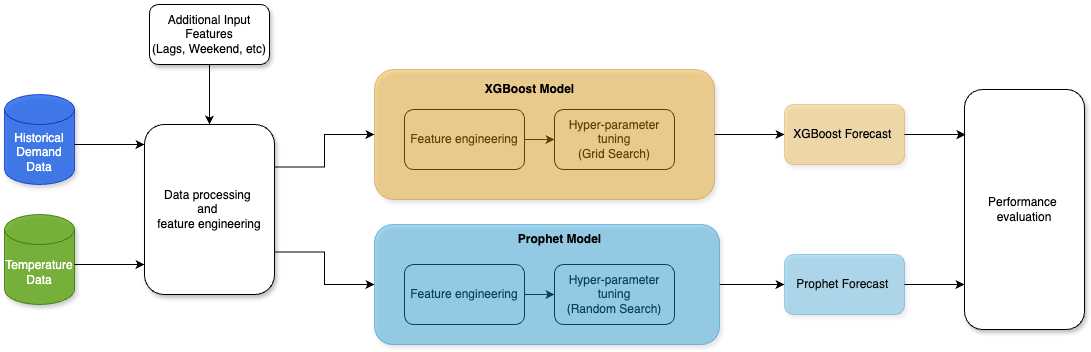
\includegraphics[width=0.80\textwidth,height=5cm]{model_diagram.png}
\caption{Model Diagram}
\label{model_diagram}
\end{figure}

\chapter{Exploratory Data Analysis}\label{exploratory-data-analysis}

Lets begin by analyzing the data to understand its characteristics.

\section{Yearly Electricity Demand}\label{yearly-electricity-demand}

Analysis of the electricity demand over the years would help identify
historic trends and any seasonal effects. As a start, lets review
average, Minimum and Maximum demand fluctuation over the years.

\begin{figure}[H]
\centering
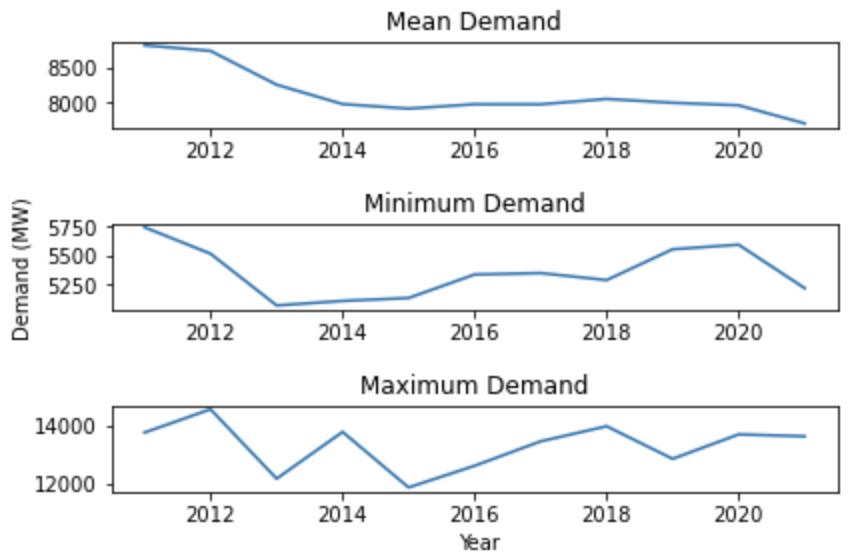
\includegraphics[width=0.80\textwidth,height=5cm]{demand_stats.png}
\caption{Yearly Demand Statistics}
\label{demand_stats}
\end{figure}

It is evident that in the Figure \ref{demand_stats} average demand has
reduced or flat lined over the years. We were expecting the demand to
rise with the population growth over the years. Therefore, it would be
prudent use latest available data for model build as we are focusing on
short term demand.

The minimum and maximum demand seem to fluctuate within a range and does
not indicate any significant trends.

\section{Decompose Time series}\label{decompose-time-series}

Electricity demand data is of time series nature. According to
Australian Energy market operator (AEMO), Time series models are more
applicable in short-term forecasting \cite{aemo2023forecasting} similar
to our research question. Time series data can be decomposed to four
components. \cite{brownlee_2017_how}

\begin{itemize}
  \item Level - The average value in the series.
  \item Trend - The increasing or decreasing value in the series.
  \item Seasonality - The repeating short-term cycle in the series.
  \item Noise - The random variation in the series.
\end{itemize}

\begin{figure}[H]
\centering
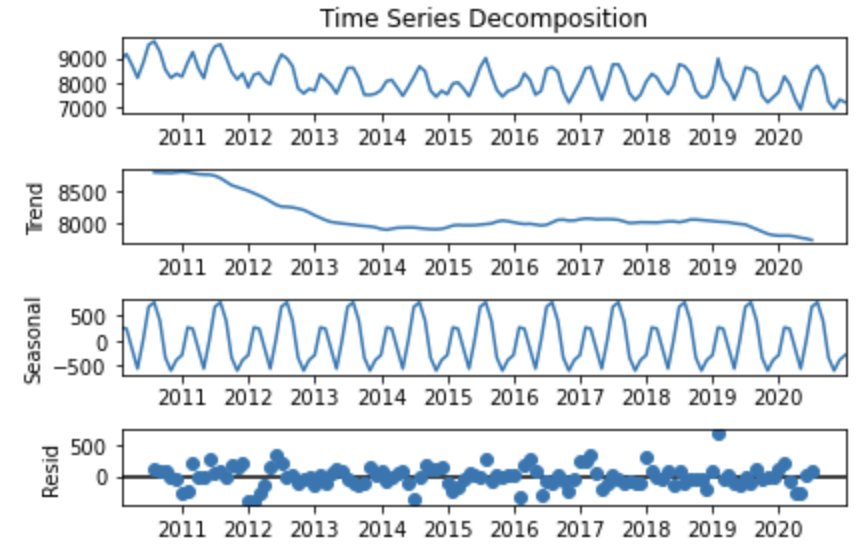
\includegraphics[width=0.80\textwidth,height=6cm]{time_series_conversion.png}
\caption{Time Series Decomposition}
\label{time_series_conversion}
\end{figure}

The Level and Trend plots both show gradual decline in demand similar to
what we observed earlier. In the Figure \ref{time_series_conversion} the
seasonal plot shows the peaks and troughs in a repetitive pattern. This
maybe due to relative high usage of electricity during Winter (for
heating) and Summer (for cooling) compared to Spring and Autumn.

Further, to verify that the data set used is suitable for time series
analysis we perform a stationarity test using ADF (Augmented
Dickey-Fuller).

The null(H0) and alternate hypothesis(H1) of ADF test are:

\begin{itemize}
  \item H0: The series has a unit root (value of a=1),the series is non-stationary.
  \item H1: The series has no unit root, the series is stationary.
\end{itemize}

If we cannot reject the null hypothesis, we can say that the series is
not stationary, and if we do, it is considered stationary.

\begin{verbatim}
## Results of Dickey-Fuller Test:
\end{verbatim}

\begin{verbatim}
## Test Statistic                   -5.586991
## p-value                           0.000001
## #Lags Used                       28.000000
## Number of Observations Used    3989.000000
## Critical Value (1%)              -3.431990
## Critical Value (5%)              -2.862265
## Critical Value (10%)             -2.567156
## dtype: float64
\end{verbatim}

Based on the results we can observe that the test statistic is lower
than the critical values. Therefore we can reject the null hypothesis
and conclude that the time series is stationary.

\section{Monthly Demand}\label{monthly-demand}

Lets analyse the impact of demand based on the month.

\begin{figure}[H]
\centering
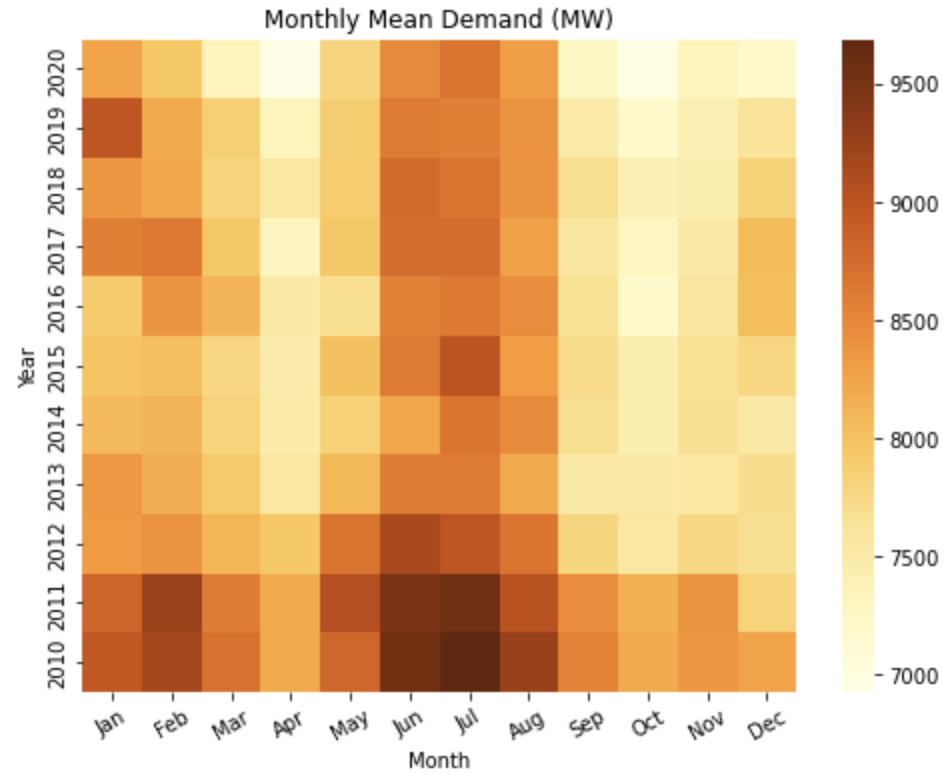
\includegraphics[width=0.80\textwidth,height=6cm]{monthly_heat.png}
\caption{Monthly Demand Heatmap}
\label{monthly_heat.png}
\end{figure}

We tend to use heating during winter months and cooling during summer.
The heatmap clearly indicates that June, July, August winter months and
January, February Summer months have a higher average demand for
electricity. Conversely Spring and Autumn has a lower average demand.
Therefore the month/season should be considered for the model build.

\section{Day of the week Demand}\label{day-of-the-week-demand}

Next we analyse whether the electricity demand fluctuate depending on
the day of the week. As per the heatmap, weekends tend to have lower
demand. This could be due to the fact that most offices, factories are
closed during the weekend. Also, many people tend to spend weekends
outside. Similar to month, day of the week seems to have an influence on
the demand. Hence suitable to be included in the model build.

\begin{figure}[H]
\centering
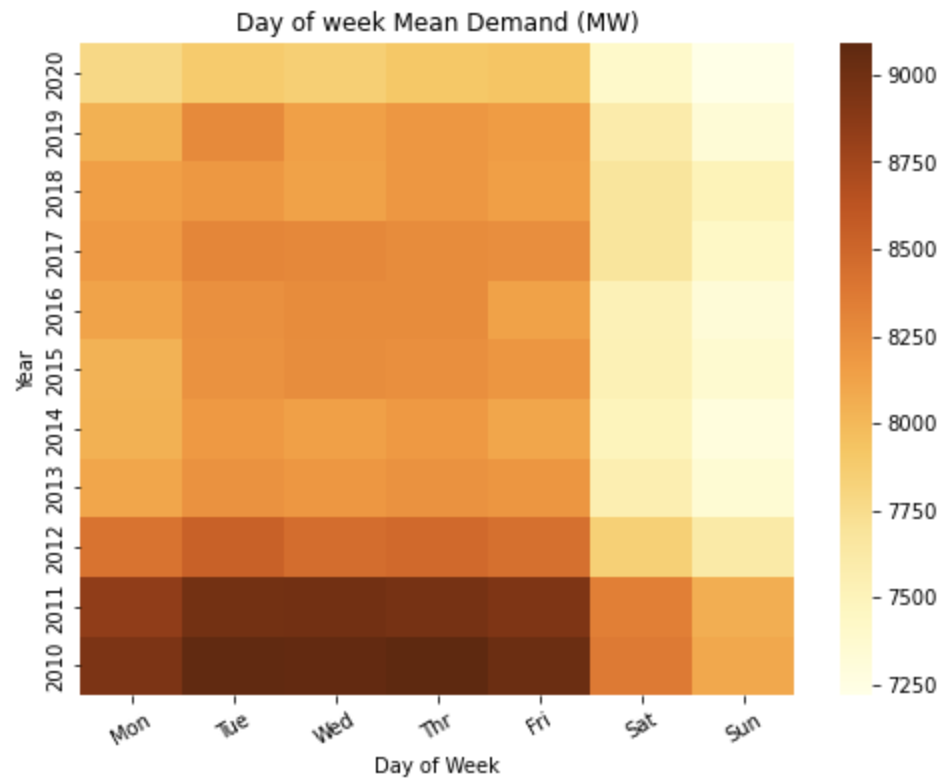
\includegraphics[width=0.80\textwidth,height=6cm]{day_heat.png}
\caption{Day of the Week Demand Heatmap}
\label{day_heat}
\end{figure}

\section{Demand on Holidays}\label{demand-on-holidays}

Extending on the day of the week demand, we would like to analyse the
difference in average demand between holidays and non-holidays. For the
purpose of the analysis, we consider Public holidays and weekends as
\textit{Holidays} and all the other days as non-holidays.

\begin{figure}[H]
\centering
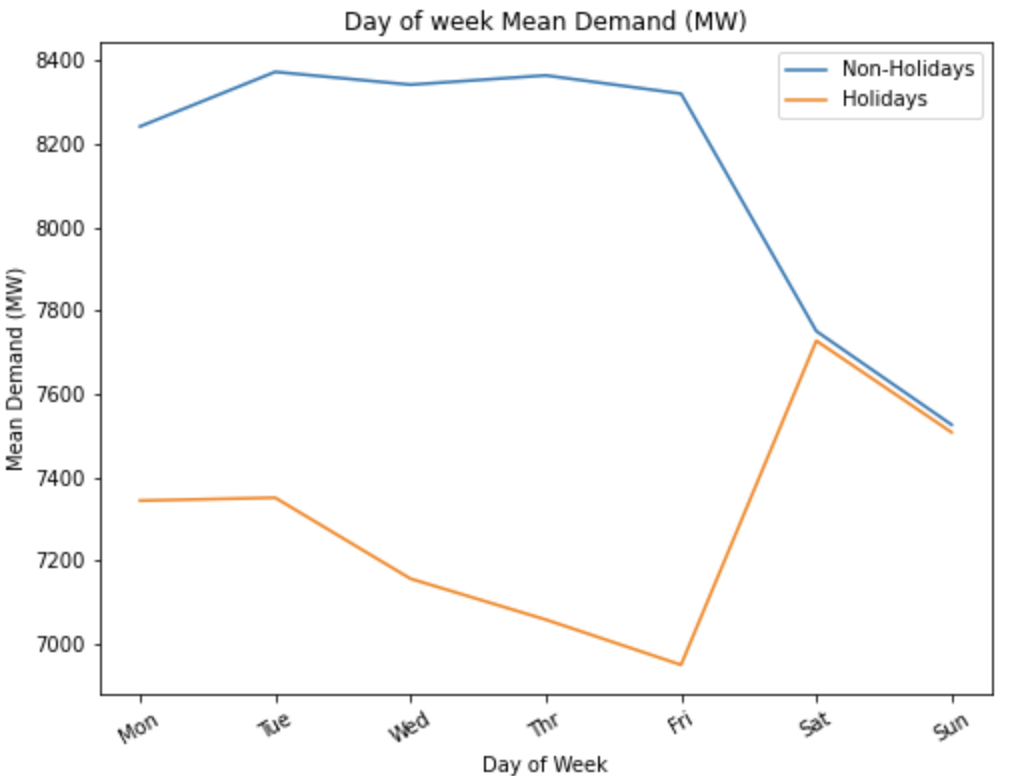
\includegraphics[width=0.80\textwidth,height=6cm]{day_demand.png}
\caption{Mean Demand Holiday vs Non-Holiday}
\label{day_demand}
\end{figure}

The graph clearly indicate a significant difference in mean demand
between holidays and non-holidays. As noted previously for Saturday and
Sunday, this may be due the fact that offices, factories not operating
over holidays resulting in lower demand. Therefore we could conclude
that holidays has a impact on the overall demand and therefore should be
considered in the model.

\section{Hour of the day demand}\label{hour-of-the-day-demand}

At the next granular level, we would like to observe how demand
fluctuates within a day (hour by hour). Australian energy providers
broadly segregates hourly demand to three groups
\cite{wrigley_2019_peak}. Peak, off-peak and shoulder. There are
variations of this by providers. For our analysis purposes, we would
simplify to Peak and Off-peak only.

\begin{figure}[H]
\centering
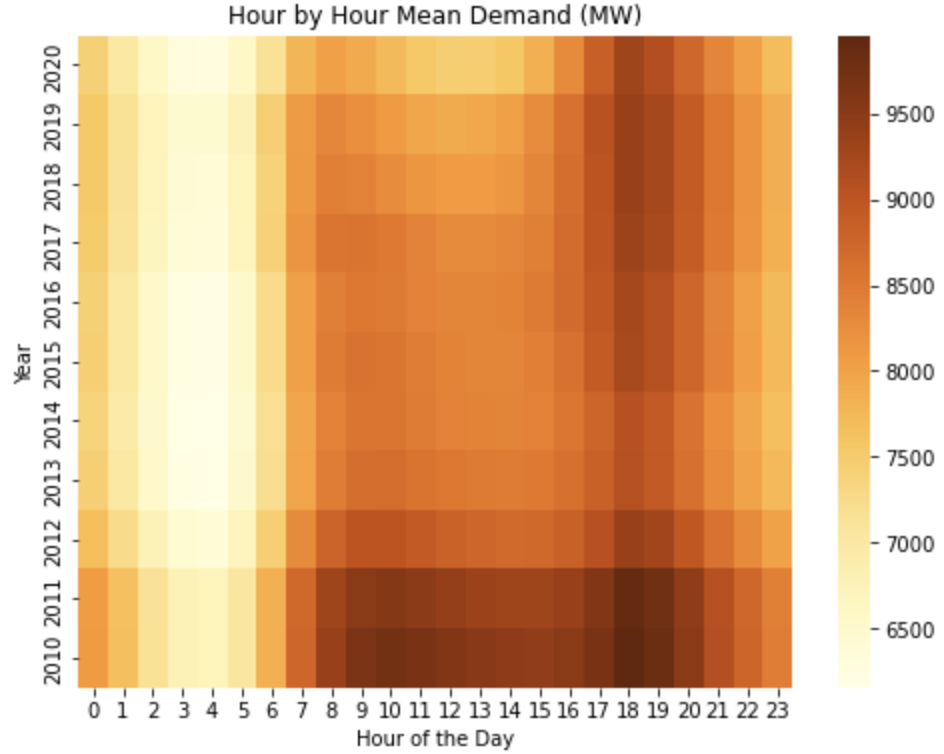
\includegraphics[width=0.80\textwidth,height=6cm]{hour_heat.png}
\caption{Hourly Demand Heatmap}
\label{hour_heat}
\end{figure}

As evident from the graph, approx from 7:00 AM to 10:00 PM, the demand
seems to be high. Therefore we would use that period as Peak demand and
rest as off-peak demand for our model build.

\section{Peak vs Off-Peak demand}\label{peak-vs-off-peak-demand}

Based on previous analysis, lets verify the variations in demand based
on Peak hours vs off-peak. Additionally, we further drill-down on
holidays vs non-holidays.

\begin{figure}[H]
\centering
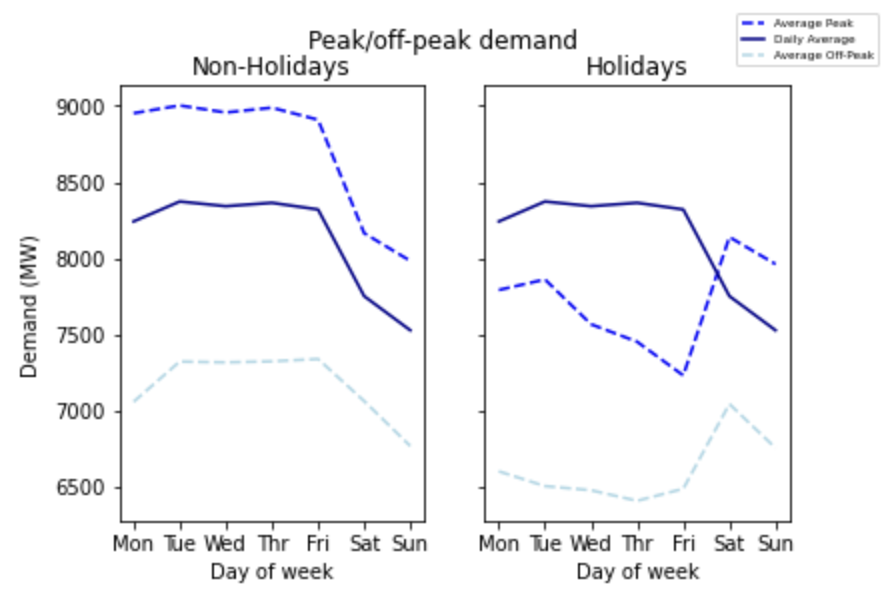
\includegraphics[width=0.80\textwidth,height=6cm]{holiday_nonholiday.png}
\caption{Peak vs Off-Peak Demand on Holiday vs Non-Holiday}
\label{holiday_nonholiday}
\end{figure}

The graphs clearly indicate the difference in demand between peak and
off-peak hours. This pattern is visible both during non-holidays and
holidays. Therefore we should consider Peak/Off-Peak demand in the model
build.

\section{Autocorrelation \& Lag}\label{autocorrelation-lag}

We would like to understand the influence of Lag in the chosen model.
Prior to that lets review the concept.

Autocorrelation (serial correlation) is correlation between two values
of the same variable at times \(t\) and \(t_k\). When a value from a
time series is regressed on previous values from that same time series,
it is referred to as an autoregressive model. e.g \(y_t\) and
\(y_{t-1}\) \[ 
y_t = \beta_0 + \beta_1 y_{t-1} + \epsilon_t
\] The above is a first order autoregressive model. Meaning only one
proceeding value is used as predictor variable and is written as AR(1).
If we used two previous values as predictors, then it would be a second
order autoregressive model i.e.~AR(2). This can be generalised as AR(k),
i.e \(k^{th}\) order autoregressive model
\cite{thepennsylvaniastateuniversity_102}.

The autocorrelation function (ACF) is given as,
\(Corr(y_t,y_{t-k}),k=1,2,..n\) \cite{nist_2020_13512} where k is the
time gap or the lag between values of the same variable. We are
interested in Partial Autocorrelation, which measure the association
between \(y_t\) and \(y_{t-k}\) directly and filter out the linear
influence of the random variables that lie in between. PACF is useful to
identify the order of autocorrelation.

\begin{figure}[H]
\centering
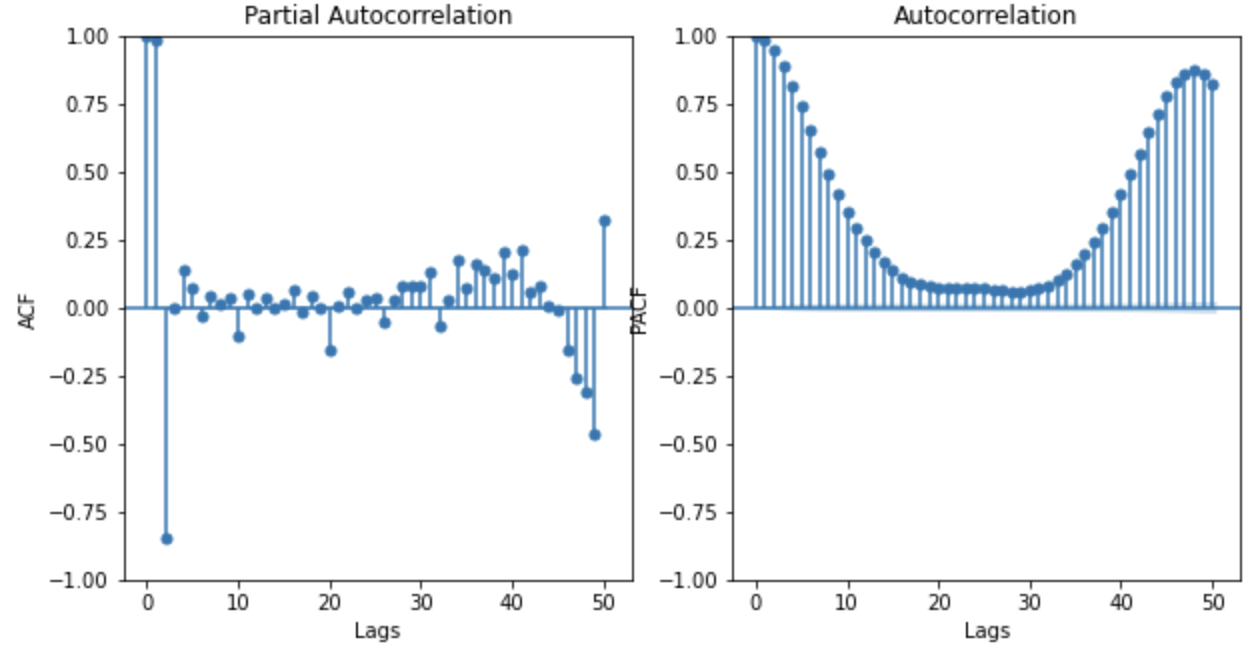
\includegraphics[width=0.80\textwidth,height=6cm]{autocorrelation.png}
\caption{Autocorrelation and Partial Autocorrelation}
\label{autocorrelation}
\end{figure}

The ACF plot seems to indicate cyclical pattern and this could be due to
seasonality effect on the demand data. It also seem to highlight high
correlation between adjacent data points.

The PACF graph shows significant spike in lag 1,2 and 3 but seems to
decay as it moves along. Hence it maybe useful to limit to 3 lags for
the model.

\section{Temperature and demand
relationship}\label{temperature-and-demand-relationship}

The relationship between temperature and electricity demand is well
known. In below grpah, as the temperature increase, it is clearly
evident that demand increases. However it is interesting to note that
when temperature decreases, especially below 10 degrees, we see a
limited spike in demand. Potential reason could be that in NSW
temperature falls mostly during the night / early morning and therefore
consumers do not necessarily need heating. However the high temperatures
are mostly during day time and as a result people use electricity for
cooling driving up the demand.

\begin{figure}[H]
\centering
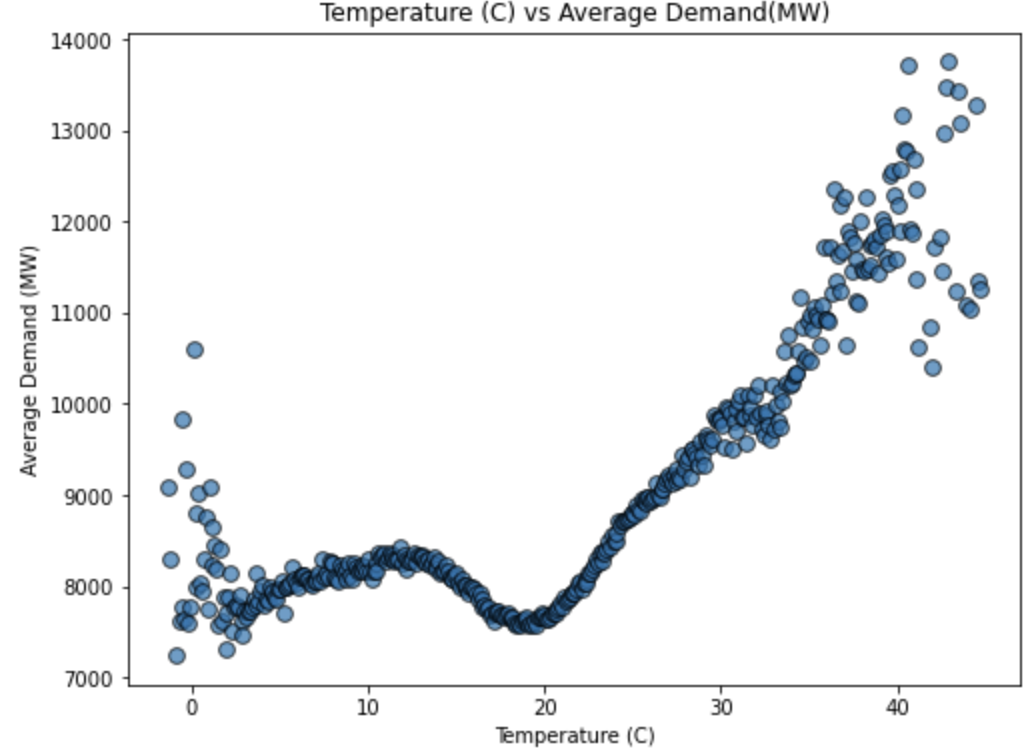
\includegraphics[width=0.80\textwidth,height=6cm]{temperature_demand.png}
\caption{Temperature vs Demand}
\label{temperature_demand}
\end{figure}

\section{Correlation matrix}\label{correlation-matrix}

Finally we look at the correlation between the attributes. The graph
below shows very low correlation between Total Demand and Temperature.
This may be due to the fact that the relationship is non-linear.
Similarly, Holiday and Month seems to have little or no correlation with
respect to demand. Hour and Peak/off-peak in turn seems to have higher
correlation.

\begin{figure}[H]
\centering
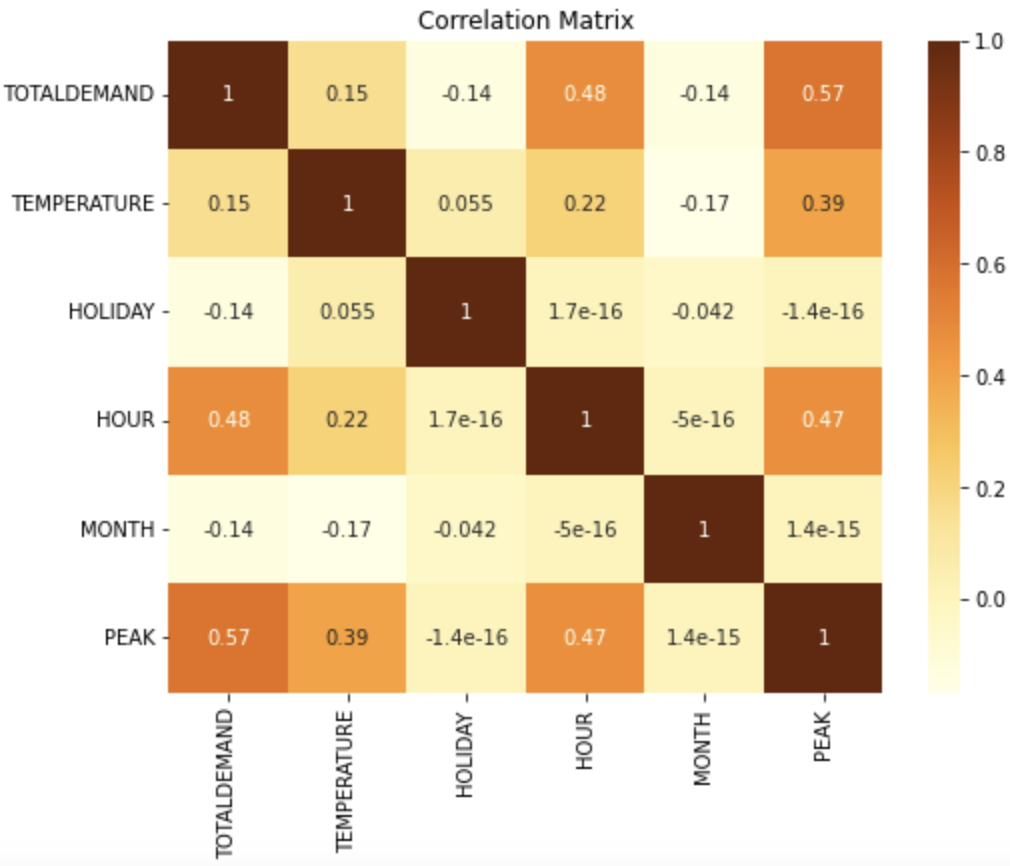
\includegraphics[width=0.80\textwidth,height=6cm]{correlation_matrix.png}
\caption{Correlation Matrix}
\label{correlation_matrix}
\end{figure}

\section{Covid impact on Demand}\label{covid-impact-on-demand}

Since the dataset used overlaps with the Covid period, it is important
to understand if there is any impact on overall demand.

\begin{figure}[H]
\centering
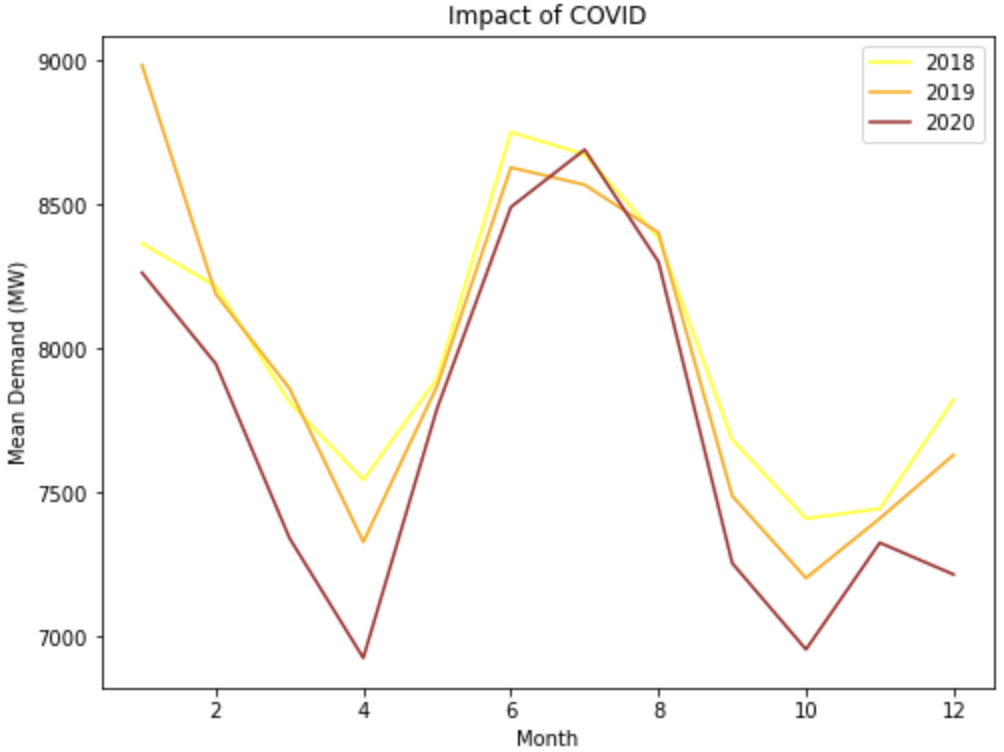
\includegraphics[width=0.80\textwidth,height=6cm]{covid_impact.png}
\caption{Covid impact on Demand}
\label{covid_impact}
\end{figure}

The plot does not indicate any significant deviations in the demand. One
could conclude that 2020 Covid period had minimal impact on overall
demand based on the graph. However, further research is warranted to
confirm the finding.

\chapter{Analysis and Results}\label{analysis-and-results}

\section{XGBoost}\label{xgboost}

\subsection{Why XGBoost}\label{why-xgboost}

XGBoost can be adjusted from standard regression to time series
regression by applying data transformations to add lag features as
predictors for the model. XGBoost is suitable for time series modelling
because of its feature engineering flexibility, high accuracy, and
ability to handle non-linear relationships
\cite{brownlee_gradientboosting2020}. XGBoost's tree-based model
structure can handle different features like categorical and continuous
variables without normalisation or scaling like other models
\cite{ambika_2023_xgboost}. This saves preprocessing time and creates a
robust model for unscaled features.

Secondly, XGBoost can capture complex non-linear relationships because
it is a decision tree-based model, and decision trees are inherently not
linear \cite{ambika_2023_xgboost}. This allows us to use as many
features as we want without worrying about feature interactions in
models like linear regression or manual feature transformations like log
or polynomial transformations.

Thirdly, XGBoost is highly accurate because of advanced algorithms and
model-building options that make it highly effective for many
machine-learning tasks \cite{ambika_2023_xgboost}. Combining boosting,
residual learning, L1 and L2 regularisation, and pruning leads to high
model accuracy. After the model is run, XGBoost shows feature importance
and allows for further hyper-parameter tuning to improve accuracy and
computational efficiency.

\subsection{How XGBoost works}\label{how-xgboost-works}

XGBoost is built upon gradient boosting, combining three elements: a
loss function that must be optimised, a weak learner to make
predictions, and an additive model to add weak learners to minimise the
loss function. Since we are tackling a time-series regression task, the
loss function is the mean Squared Error
\cite{brownlee_gradientboosting2020}.

The weak learner in XGBoost is a decision tree, but not a complex
decision tree like random forests. XGBoost uses shallow trees with
limited depth as weak learners. The trees are weak predictors but can be
used to create an accurate model combined. An XGBoost decision tree is
different from the typical decision tree. XGBoost uses the gradient and
Hessian (a second-order measure of the curvature of the loss function)
to improve the model, which is a further improvement over improving the
model using gradient only \cite{chen_2016_xgboost}.

The goal is to predict the total demand from the given features. First,
each row's total demand average and residuals are calculated. Next, a
similar score is calculated using the formula below. Lambda is a
regularisation parameter that prevents overfitting by penalising overly
complex trees and encouraging them to split only when significant
improvement occurs \cite{chen_2016_xgboost}.

\[
\text{Similarity Score} = \frac{\sum{(residuals)}^2 }{\text{number of residuals} + \lambda}
\]

The intuition behind the similarity score is to determine whether to
split the data at a specific leaf. The goal is to determine whether
splitting at a particular leaf will improve the predictive power by
grouping similar residuals.

The Gain Score will be used to determine whether a split is good.

\[
Gain = {Similarity}_{left} + {Similarity}_{right} - {Similarity}_{root}
\]

The similarity score for the root and leaf nodes can be calculated, and
the Gain formula can be applied. We can test different thresholds by
comparing Gain from different thresholds. The higher the gain score, the
better the threshold for splitting residuals into clusters of similar
values. Once the best threshold for splitting is determined, the same
process is applied to the leaves; to prevent overfitting, a max tree
depth can be set in the model parameters. Max tree depth and lambda can
both help reduce overfitting. The above process is run until the max
tree depth or no more residuals are split \cite{a2016_how}.

The next step is to prune the trees we made. A value Gamma is chosen,
and we subtract the gain of each branch by Gamma. If the result is
negative, that branch doesn't provide enough improvement, so the branch
is pruned. The lambda decreases the similarity score, hence decreasing
the Gain value. A smaller Gain value means it is easier to prune
branches and even whole trees \cite{a2016_how}.

\subsection{Predicting Values}\label{predicting-values}

Prediction formula (Sneha, 2020): \[
\text{Predicted values} = \text{Average total demand} + \text{Learning rate} * \text{Average of each leaf}
\] For example, the initial prediction is that the average total demand
is 7,000 MW, and the learning rate is 0.3. The first observation had a
temperature of 20, so the average of that leaf was -25. The predicted
value is: \[
7,000 + (0.3 \times (-25)) = 6,993
\] The process is repeated for each value we want to predict, and the
residuals are calculated again, repeating until the maximum number of
trees is reached or the model does not improve.

\subsection{Model Specifications}\label{model-specifications}

Electricity demand patterns change over time due to technological
shifts, economic factors, and consumer behaviour. Using recent data, our
model will capture recent trends and behaviours and provide more
accurate forecasts. The model should be exposed to an equal number of
seasons to capture the seasonal variations and differences in
consumption patterns throughout the year. For computational efficiency,
a subset of the data will be used to efficiently reduce run time and
tune hyperparameters. Based on the factors above, the data range chosen
for the model will start in April 2018 and continue until March 2021.

\subsection{Train Test Split}\label{train-test-split}

The train-test split is done differently in a time series regression
model. Firstly, the chosen dataset is ordered chronologically to
preserve the temporal order of the data. Eighty percent of the
chronologically ordered data is used for training, and the remainder for
testing \cite{brownlee_2020_how}.

The Fig \ref{traintest} illustrates a time series train-test split. The
blue colour shows the data used for training, while the orange is the
testing data. The stripped line represents the transition from training
to testing.

\begin{figure}[H]
\centering
\includegraphics[width=0.95\textwidth, height=5cm]{traintest.png}
\caption{Train-Test Split for XGBoost Model}\label{traintest}
\end{figure}

\subsection{Hyperparameter Tuning}\label{hyperparameter-tuning}

Hyperparameter tuning is critical to improving model accuracy. The two
methods considered for tuning are Grid Search and Random Search. Grid
Search is an exhaustive search testing all possible combinations for
hyperparameter values. Random Search randomly samples a fixed number of
hyperparameter combinations. The trade-off is finding the best
combination of hyperparameters vs.~computational efficiency. Random
Search is chosen due to computational constraints.

The first hyperparameter is the number of trees (n\_estimators) the
model can build. A more significant number of trees allows the model to
capture more complex patterns but increases the risk of overfitting and
longer training time. The tuning range for the number of trees is
{[}100,200,300,500{]}, allowing for a gradual increase in trees for
balanced exploration of a simple model with a few trees and complex
models with many trees. Tree addition has diminishing returns; after a
certain number of trees, only computational cost will increase, but
model performance will plateau \cite{a2022_xgboost}.

The learning rate determines how much each tree contributes to the final
prediction. A lower learning rate means the model learns slower and has
a higher training time. While a significant learning rate means the
model will learn fast using less computational power, it is more prone
to overfitting. The small learning rate (0.01) allows the model to
capture underlying patterns, but convergence is slow. The low learning
rate(0.05) uses fewer trees but is still enough to prevent overfitting.
This value balances run time and model accuracy \cite{a2022_xgboost}.

The standard learning rate (0.1) is usually used as a benchmark to
compare lower or higher learning rates. The high learning rate (0.3)
helps reduce training time, but with a high convergence speed, the model
will have a high variance. The high learning rates are explored to
determine whether faster learning provides better results or leads to
overfitting. The max depth hyperparameter controls the depth of each
tree. Deeper trees are better at capturing more complex patterns but
have a higher risk of overfitting. The tree depth has the same rationale
as the learning rate with shallow trees (3), medium depth (5), increased
depth (7), and deep trees (10). The trade-offs are the same between
bias, variance, overfitting, and computational efficiency
\cite{a2022_xgboost}.

The gamma parameter (Lambda) in XGBoost is a regularisation parameter
that prevents the model from overfitting. No regularisation (0) means no
tree-splitting restrictions, capturing detailed patterns. No
regularisation serves as a base for comparing regularisation levels.
Medium regularisation (0.1) allows only significant splits, which leads
to better generalisation and a balance between complexity and pruning.
High regularisation (0.3) focuses on essential splits and improves model
simplicity \cite{a2022_xgboost}.

The random search uses 50 iterations for computational efficiency. Each
iteration takes a combination of random values from each hyperparameter
list and tests the performance. The lowest mean squared error determines
the best model. Sci-kit, by default, tries to maximise scores, so
setting a negative mean squared error addresses that issue.

Cross-validation is done differently in time series. The
\texttt{TimeSeriesSplit} ensures that the training happens on past data
and tests on future data based on past information to preserve the
temporal aspect of the time series \cite{scikit-learn2024}. The best
results after a random search are:

\begin{Shaded}
\begin{Highlighting}[]
\NormalTok{Best Parameters: \{}\StringTok{\textquotesingle{}n\_estimators\textquotesingle{}}\NormalTok{: }\DecValTok{300}\NormalTok{, }
                  \StringTok{\textquotesingle{}max\_depth\textquotesingle{}}\NormalTok{: }\DecValTok{5}\NormalTok{, }
                  \StringTok{\textquotesingle{}learning\_rate\textquotesingle{}}\NormalTok{: }\FloatTok{0.1}\NormalTok{, }
                  \StringTok{\textquotesingle{}gamma\textquotesingle{}}\NormalTok{: }\FloatTok{0.3}\NormalTok{\}}
\end{Highlighting}
\end{Shaded}

\subsection{Diagnostic Plots}\label{diagnostic-plots}

\subsubsection{Feature Imporance}\label{feature-imporance}

The F score represents the number of times a feature is used to split
data. The higher the f-score, the more critical a feature is to the
model. The most essential features are Temperature, lag, and hour. The
model is not too reliant on one feature, as the top three features have
very close F scores. Temperature is expected to have a significant
impact, as observed in the literature. Lag 1, the previous demand for
the last 30 minutes, is expected to contribute significantly to a time
series regression model. Three lag features provided the maximum model
improvement.

The hour is transformed using the cosine function to address the issue
of hour proximity \cite{avanwyk_2022_encoding}. For example, if we have
hour ``23,'' hour ``00,'' and hour ``05,'' the model might assume that
hour ``05'' is closer to hour ``00,'' but that is false. The cosine
transformation will address this issue, giving peak hours more
significance.

The hour has a significant impact and captures the effect of intraday
demand. The seasons are one-hot encoded, so the interpretation differs
from numerical values. The most important features are the closest to
the time interval forecasted.

\begin{figure}[H]
\centering
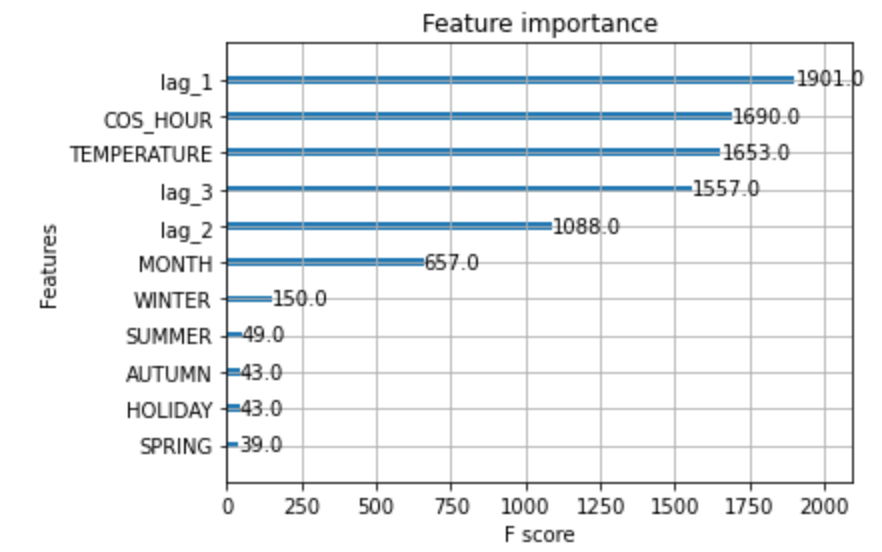
\includegraphics[width=0.95\textwidth, height=5cm]{featureimp.png}
\caption{Feature Importance for XGBoost Model}\label{featureimp}
\end{figure}

\subsubsection{Actual \& Predicted
Values}\label{actual-predicted-values}

The Figure \ref{actualpredict} shows an upward-sloping diagonal line,
which indicates that the model did an excellent job predicting the
target variable.

\begin{figure}[H]
\centering
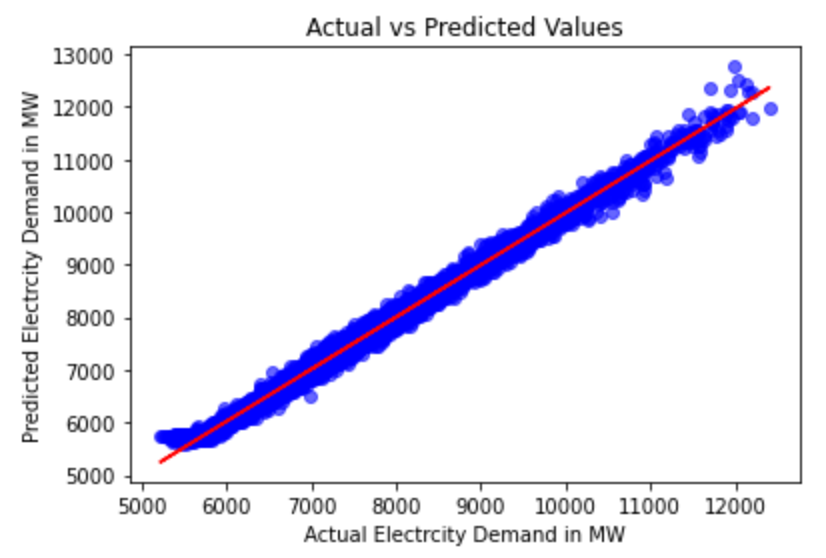
\includegraphics[width=0.95\textwidth, height=5cm]{actualpredict.png}
\caption{Feature Importance for XGBoost Model}\label{actualpredict}
\end{figure}

\subsubsection{Model Results}\label{model-results}

The two metrics used to measure performance are root mean squared error
(RMSE) and mean absolute error (MAE).

\begin{Shaded}
\begin{Highlighting}[]
\NormalTok{Root Mean Squared Error : }\FloatTok{95.43}
\NormalTok{Mean Absolute Error: }\FloatTok{70.77}
\NormalTok{Mean Absolute Percentage Error: }\DecValTok{1}\OperatorTok{\%}
\end{Highlighting}
\end{Shaded}

The RMSE measures the average size of the error between the actual and
predicted values. An RMSE of 95.84 means that, on average, the predicted
values are off by 95.84MW. The MAE measures the average of the absolute
difference between the actual and predicted values. MAE is more robust
against outliers because it does not square the error. An MAE of 70.86
means that, on average, the model is off by 70.86MW. The MAPE is 1\% of
the target range (5000 MW---13000 MW). This suggests that the model is
performing reasonably well.

\subsection{Forecasting}\label{forecasting}

The last 17 days of the dataset will be forecasted using the XGBoost and
Prophet models to compare with the provided AEMO forecasted demand.

\begin{Shaded}
\begin{Highlighting}[]
\NormalTok{RMSE: }\FloatTok{232.56}
\NormalTok{MAE: }\FloatTok{160.14}
\NormalTok{MAPE: }\FloatTok{2.0}\OperatorTok{\%}
\end{Highlighting}
\end{Shaded}

XGBoost and Facebook Prophet had lower errors compared to the AEMO
forecast model. Since both RMSE and MAE are lower for XGBoost and
Facebook Prophet, Both models generally perform better across small and
large errors. The plot below shows how the models predicted actual
demand. We can see that XGBoost follows the actual demand more closely.

\begin{figure}[H]
\centering
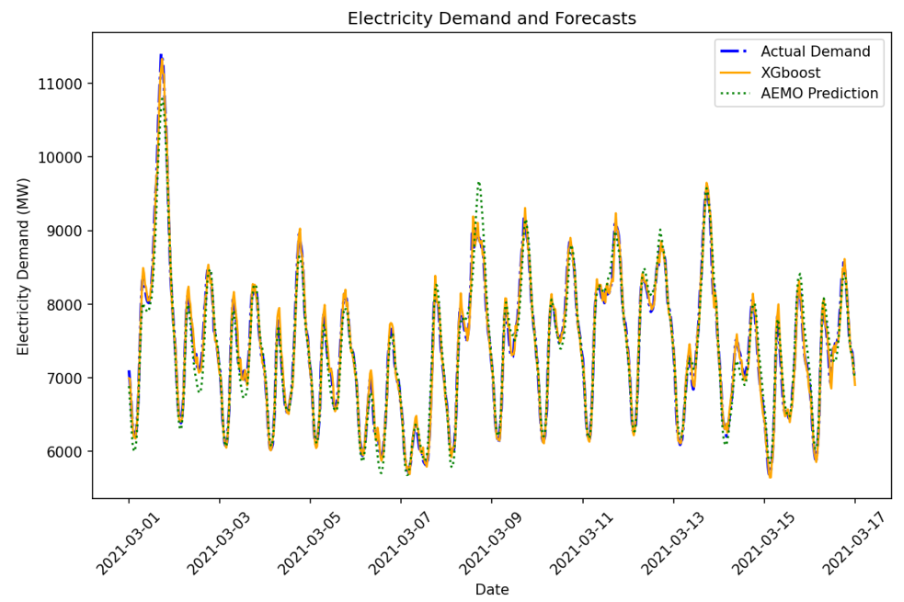
\includegraphics[width=0.95\textwidth, height=5cm]{forecastplot.png}
\caption{Forecast plot of XGBoost Model}\label{forecastplot}
\end{figure}

\section{Facebook Prophet}\label{facebook-prophet}

\subsection{Model Specifications}\label{model-specifications-1}

Prophet was developed internally at Facebook (now known as Meta) to
optimally handle business forecasting tasks, which typically features
multiple seasonality, missing data, and outliers
\cite{taylor2017facebook}. Prophet is a decomposable time series model
with three main components: trend, seasonality, and holidays. The trend
component models non-periodic changes in the value of the time series.
The seasonality component models periodic changes in the value of the
time series. The holiday component models the effects of holidays that
occur on potentially irregular schedules over one or more days. The
model is fitted to historical data, and future data is forecasted using
the model. The model is highly customisable, allowing users to adjust
the model to fit their data and business needs. This model is a
regression model with interpretable parameters that can be intuitively
adjusted by analysts with domain knowledge about the time series. In the
proposed Prophet model, they use a decomposable time series model with
three main model components: trend, seasonality, and holidays. They are
combined in the following equation:

\[
y(t) = g(t) + s(t) + h(t) + \epsilon_t
\]

Here \(g(t)\) is the trend function which models non-periodic changes in
the value of the time series, \(s(t)\) represents periodic changes
(e.g., weekly and yearly seasonality), and \(h(t)\) represents the
effects of holidays which occur on potentially irregular schedules over
one or more days. The error term represents any idiosyncratic changes
which are not accommodated by the model; they make the parametric
assumption that \(t\) is normally distributed.

This specification is similar to a generalized additive model (GAM), a
class of regression models with potentially non-linear smoothers applied
to the regressors. Here we use only time as a regressor but possibly
several linear and non-linear functions of time as components. Modelling
seasonality as an additive component is the same approach taken by
exponential smoothing. Multiplicative seasonality, where the seasonal
effect is a factor that multiplies \(g(t)\), can be accomplished through
a log transform.

The growth is typically modeled as a logistic growth curve, which is a
common pattern in many business time series. The logistic growth model
has an inflection point that can be used to model changes in growth
rates. The logistic growth curve is defined as:

\[
g(t) = \frac{C}{1 + \exp(-k(t - m))}
\] Where \(C\) is the carrying capacity of the growth, \(k\) is the
growth rate, and \(m\) is the offset prarameter. The trend component
models the non-periodic changes in the value of the time series. The
model also provides a piecewise linear or logistic growth curve, which
is useful for modeling growth that changes over time. The growth can be
adjusted by adding changepoints at which the growth rate is allowed to
change. The changepoints are selected automatically by the model, but
the user can also specify them manually. The changepoints are selected
by fitting a linear or logistic regression to the data and then using a
regularized optimization procedure to select the changepoints. The trend
model for changepoint is:

\[
g(t) = (k+a(t)^T\delta) t + (m+a(t)^T\gamma)
\]

Where as mentioned earlier, \(k\) is the growth rate, \(\delta\) is the
rate adjustments, and \(m\) is the offset parameter. \(\gamma_j\) is set
to \(-s_j\delta_j\) to make the function continuous.

Business time series often have multi-period seasonality as a result of
the human behaviours they represent. For instance, a 5-day work week can
produce effects on a time series that repeat each week, while vacation
schedules and school breaks can produce effects that repeat each year.
To fit and forecast these effects we must specify seasonality models
that are periodic functions of \(t\). In the model, they rely on Fourier
series to provide a flexible model of periodic effects. Let P be the
regular period we expect the time series to have (e.g.~P = 365.25 for
yearly data or P = 7 for weekly data, when we scale our time variable in
days). We can approximate arbitrary smooth seasonal effects with: \[
s(t) = \sum_{n=1}^{N} (a_n \cos(\frac{2\pi nt}{P}) + b_n \sin(\frac{2\pi nt}{P}))
\]

Seasonalities are estimated using a partial Fourier sum. The number of
terms in the partial sum (the order) is a parameter that determines how
quickly the seasonality can change. The default Fourier order for yearly
seasonality is 10, which produces this fit. The default values are often
appropriate, but they can be increased when the seasonality needs to fit
higher-frequency changes, and generally be less smooth. The Fourier
order can be specified for each built-in seasonality when instantiating
the model. Increasing the number of Fourier terms allows the seasonality
to fit faster changing cycles, but can also lead to overfitting.

Holidays and events provide large, somewhat predictable shocks to many
business time series and often do not follow a periodic pattern, so
their effects are not well modeled by a smooth cycle. As with
seasonality, we use a prior \(\kappa \sim {N(0,\nu)}\).

Prophet will by default fit weekly and yearly seasonalities, if the time
series is more than two cycles long. It will also fit daily seasonality
for a sub-daily time series. We can add other seasonalities (monthly,
quarterly, hourly) using the \texttt{add\_seasonality} method.

In this section, we will discuss the implementation of the Facebook
Prophet model for short-term electricity demand forecasting. As we have
already discussed in the earlier section that Facebook Prophet is a
powerful tool for time series forecasting that can handle multiple
seasonalities, holidays, and missing data. We will walk through the
steps of data pre-processing, model parameter tuning, and
cross-validation to evaluate the model's performance.

\subsection{Data pre-processing}\label{data-pre-processing}

Prophet follows the sklearn model API structure, where we first create
an instance of the \texttt{Prophet} class and then use its \texttt{fit}
and \texttt{predict} methods.

The input for Prophet must always be a DataFrame containing two specific
columns: \texttt{ds} and \texttt{y}. The \texttt{ds} column
(representing the date) should be in a format recognized by Pandas, such
as \texttt{YYYY-MM-DD} for a date or \texttt{YYYY-MM-DD\ HH:MM:SS} for a
timestamp. So we have changed our \texttt{DATETIME} column to
\texttt{ds}. The \texttt{y} column should be containing numeric values
representing the variable we want to forecast, thus we change the
\texttt{DEMAND} column to \texttt{y} column.

\subsection{Hyper-parameter tuning}\label{hyper-parameter-tuning}

For the model prophet it is recommended to tune the parameters like -
\linebreak \texttt{changepoint\_prior\_scale},
\texttt{seasonality\_prior\_scale}, \texttt{holidays\_prior\_scale}, and
\texttt{seasonality\_mode}. We have considered the following parameters
for tuning:

\begin{itemize}
\item
  \texttt{seasonality\_prior\_scale} parameter controls the flexibility
  of the seasonality. Similarly, a large value allows the seasonality to
  fit large fluctuations, a small value shrinks the magnitude of the
  seasonality. The default is 10., which applies basically no
  regularization.
\item
  \texttt{holidays\_prior\_scale} parameter controls flexibility to fit
  holiday effects. It also defaults to 10.0 which applies basically no
  regularization, since we usually have multiple observations of
  holidays and can do a good job of estimating their effects. This could
  also be tuned on a range of {[}0.01, 10{]} as with
  seasonality\_prior\_scale which we decide based on the grid search
  results that is discussed later.
\item
  \texttt{seasonality\_mode} parameter options are
  {[}\texttt{\textquotesingle{}additive\textquotesingle{}},
  \texttt{\textquotesingle{}multiplicative\textquotesingle{}}{]}.
  Default is \texttt{\textquotesingle{}additive\textquotesingle{}}. This
  is best identified just from looking at the time series of our data
  and we observe that the seasonal fluctuations are roughly constant in
  size over time, so we consider using additive seasonality.
\end{itemize}

Prophet does not have a built in grid search method so we have used
\texttt{sklearn} the \texttt{ParameterGrid} method from the
\texttt{sklearn} library to tune the hyper-parameters. We have specified
the grid parameters and run the grid search. We have used. We have used
the \texttt{mean\_squared\_error} as the scoring parameter for the grid
search. The best parameters are selected based on the lowest mean
squared error.

\begin{Shaded}
\begin{Highlighting}[]
\NormalTok{Best Parameters: \{}\StringTok{\textquotesingle{}daily\_seasonality\textquotesingle{}}\NormalTok{: }\VariableTok{True}\NormalTok{, }
                  \StringTok{\textquotesingle{}holidays\_prior\_scale\textquotesingle{}}\NormalTok{: }\FloatTok{0.1}\NormalTok{, }
                  \StringTok{\textquotesingle{}seasonality\_mode\textquotesingle{}}\NormalTok{: }\StringTok{\textquotesingle{}additive\textquotesingle{}}\NormalTok{, }
                  \StringTok{\textquotesingle{}seasonality\_prior\_scale\textquotesingle{}}\NormalTok{: }\FloatTok{1.0}\NormalTok{, }
                  \StringTok{\textquotesingle{}weekly\_seasonality\textquotesingle{}}\NormalTok{: }\VariableTok{True}\NormalTok{, }
                  \StringTok{\textquotesingle{}yearly\_seasonality\textquotesingle{}}\NormalTok{: }\VariableTok{True}\NormalTok{\}}
\end{Highlighting}
\end{Shaded}

\subsection{Model parameter}\label{model-parameter}

We are considering holidays in our model, so we need to create a
dataframe for them. It has two columns (\texttt{holiday} and
\texttt{ds}) and a row for each occurrence of the holiday. It includes
all occurrences of the holiday, both in the past (back as far as the
historical data go) and in the future (out as far as the forecast is
being made). We have included columns \texttt{lower\_window} and
\texttt{upper\_window} which extend the holiday out to
\texttt{{[}lower\_window,\ upper\_window{]}} days around the date. For
example, we wanted to include Christmas eve and Boxing day in addition
to Christmas day we need to include
\texttt{lower\_window=-1,upper\_window=1}.

Final model parameters:

\begin{Shaded}
\begin{Highlighting}[]
\NormalTok{model }\OperatorTok{=}\NormalTok{ Prophet(daily\_seasonality }\OperatorTok{=} \VariableTok{True}\NormalTok{, }
\NormalTok{                weekly\_seasonality}\OperatorTok{=}\VariableTok{False}\NormalTok{, }
\NormalTok{                yearly\_seasonality}\OperatorTok{=}\VariableTok{True}\NormalTok{,   }
\NormalTok{                holidays}\OperatorTok{=}\NormalTok{holiday\_nsw\_2018\_2021, }
\NormalTok{                holidays\_prior\_scale}\OperatorTok{=}\FloatTok{0.1}\NormalTok{, }
\NormalTok{                seasonality\_prior\_scale}\OperatorTok{=}\DecValTok{10}\NormalTok{)}
\end{Highlighting}
\end{Shaded}

Additional regressors are used in the model and they are added to the
linear part of the model using the \texttt{add\_regressor} method. Based
on the literature review, EDA and experimentation we have considered the
following regressors for the Prophet model to forecast demand:

\begin{itemize}
\item
  Continuous variable: \texttt{TEMPERATURE}, \texttt{lag\_1},
  \texttt{lag\_2}, \texttt{lag\_3}
\item
  Binary variable: \texttt{SUMMER}, \texttt{AUTUMN}, \texttt{WINTER},
  \texttt{SPRING}
\end{itemize}

We these parameters in the model as additional regressors :

\begin{Shaded}
\begin{Highlighting}[]
\NormalTok{[}\StringTok{\textquotesingle{}TEMPERATURE\textquotesingle{}}\NormalTok{,}\StringTok{\textquotesingle{}SUMMER\textquotesingle{}}\NormalTok{, }\StringTok{\textquotesingle{}AUTUMN\textquotesingle{}}\NormalTok{, }\StringTok{\textquotesingle{}WINTER\textquotesingle{}}\NormalTok{, }\StringTok{\textquotesingle{}SPRING\textquotesingle{}}\NormalTok{, }
        \StringTok{\textquotesingle{}lag\_1\textquotesingle{}}\NormalTok{, }\StringTok{\textquotesingle{}lag\_2\textquotesingle{}}\NormalTok{, }\StringTok{\textquotesingle{}lag\_3\textquotesingle{}}\NormalTok{]}
\end{Highlighting}
\end{Shaded}

\subsection{Cross-Validation}\label{cross-validation}

The traditional method to tune model's performance is the
\textbf{hold-out} validation that splits the whole dataset in to
training validation and test set. We have applied 80/20 split for
training and testing. The model is trained on the train set and
performance is evaluated on test set.

As mentioned in the literature review that we consider forward-chaining
cross validation, we perform 5-fold cross validation for a range of
historical cutoffs using the \texttt{cross\_validation} function. We
have used \texttt{cutoffs} keyword \texttt{cross\_validation\ function}
and specify the custom cutoffs.

In the Fig \ref{cross_validation_output} we have shown the terminology
used in the cross-validation method. - \texttt{initial} is the first
training period. In Fig \ref{cross_validation_output}, it would be the
first two blocks of data in the first fold. It is the minimum amount of
data needed to begin the training and we need to at least have 365.6
days of data. Considering our dataset we have used 14 months as
\texttt{initial} parameter. the first fold to capture the yearly
seasonality. - \texttt{horizon} is the length of time we want to
evaluate the forecast over, in this case we have set the horizon to 15
days. - \texttt{period} is the amount of time between each fold. We have
used approximately 7 months as the period. - \texttt{cutoffs} are the
dates when each horizon will begin.

\begin{figure}[H]
\centering
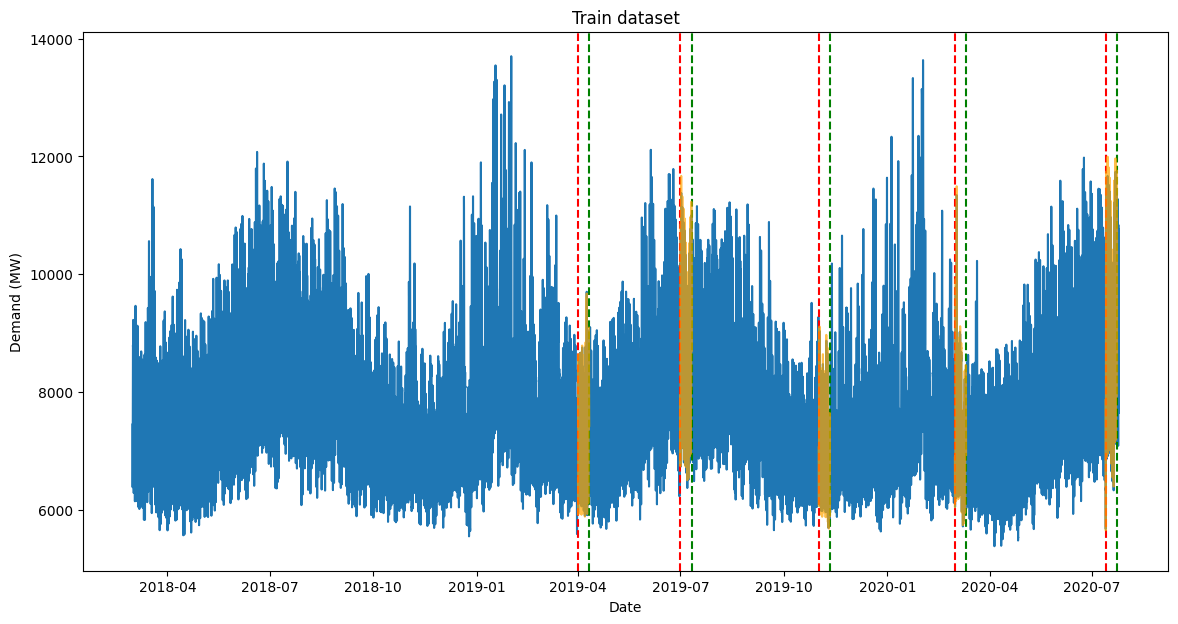
\includegraphics[width=0.95\textwidth, height=5cm]{cross_validation_output.png}
\caption{Cross-validation terminology}\label{cross_validation_output}
\end{figure}

\subsection{Model Results}\label{model-results-1}

Below is the result of the Prophet model:

\begin{Shaded}
\begin{Highlighting}[]
\NormalTok{Root Mean Squared Error: }\FloatTok{111.5663}
\NormalTok{Mean Absolute Error: }\FloatTok{87.6737}
\NormalTok{Mean Absolute Percentage Error: }\FloatTok{0.0118}
\end{Highlighting}
\end{Shaded}

The model has performed well in forecasting the electricity demand for
the test data. The MAPE is 0.0118 which is 1.18\% and indicates that the
model is performing well.

The result of cross validation:

\begin{Shaded}
\begin{Highlighting}[]
\NormalTok{    Cutoff      MSE           RMSE          MAE         MAPE}
\DecValTok{0}   \DecValTok{2019}\OperatorTok{{-}}\DecValTok{0}\ErrorTok{4}\OperatorTok{{-}}\DecValTok{0}\ErrorTok{1}  \FloatTok{6730.187098}   \FloatTok{82.037718}     \FloatTok{61.726130}   \FloatTok{0.008176}
\DecValTok{1}   \DecValTok{2019}\OperatorTok{{-}}\DecValTok{0}\ErrorTok{7}\OperatorTok{{-}}\DecValTok{0}\ErrorTok{1}  \FloatTok{14260.09658}   \FloatTok{119.41565}     \FloatTok{85.875777}   \FloatTok{0.009713}
\DecValTok{2}   \DecValTok{2019}\OperatorTok{{-}}\DecValTok{11}\OperatorTok{{-}}\DecValTok{0}\ErrorTok{1}  \FloatTok{7165.935874}   \FloatTok{84.651851}     \FloatTok{65.489314}   \FloatTok{0.009165}
\DecValTok{3}   \DecValTok{2020}\OperatorTok{{-}}\DecValTok{0}\ErrorTok{3}\OperatorTok{{-}}\DecValTok{0}\ErrorTok{1}  \FloatTok{6782.806298}   \FloatTok{82.357794}     \FloatTok{64.052253}   \FloatTok{0.008441}
\DecValTok{4}   \DecValTok{2020}\OperatorTok{{-}}\DecValTok{0}\ErrorTok{7}\OperatorTok{{-}}\DecValTok{13}  \FloatTok{17569.08641}   \FloatTok{132.54843}     \FloatTok{96.610446}   \FloatTok{0.010811}
\end{Highlighting}
\end{Shaded}

The cross-validation results show that the model has performed well for
almost all the cutoffs. The MAPE is also close to 1\% for all the
cutoffs which indicates that the model is performing well.

The Fig \ref{prophet_component_plot} shows the trend and seasonality
components of the model. The trend component shows the overall trend of
the electricity demand, while the seasonality component shows the daily
and weekly seasonality patterns. The holidays component shows the impact
of holidays on the electricity demand. As we have predicted the
\texttt{yearly} seasonality shows the summer and winter spike.

\begin{figure}[H]
\centering
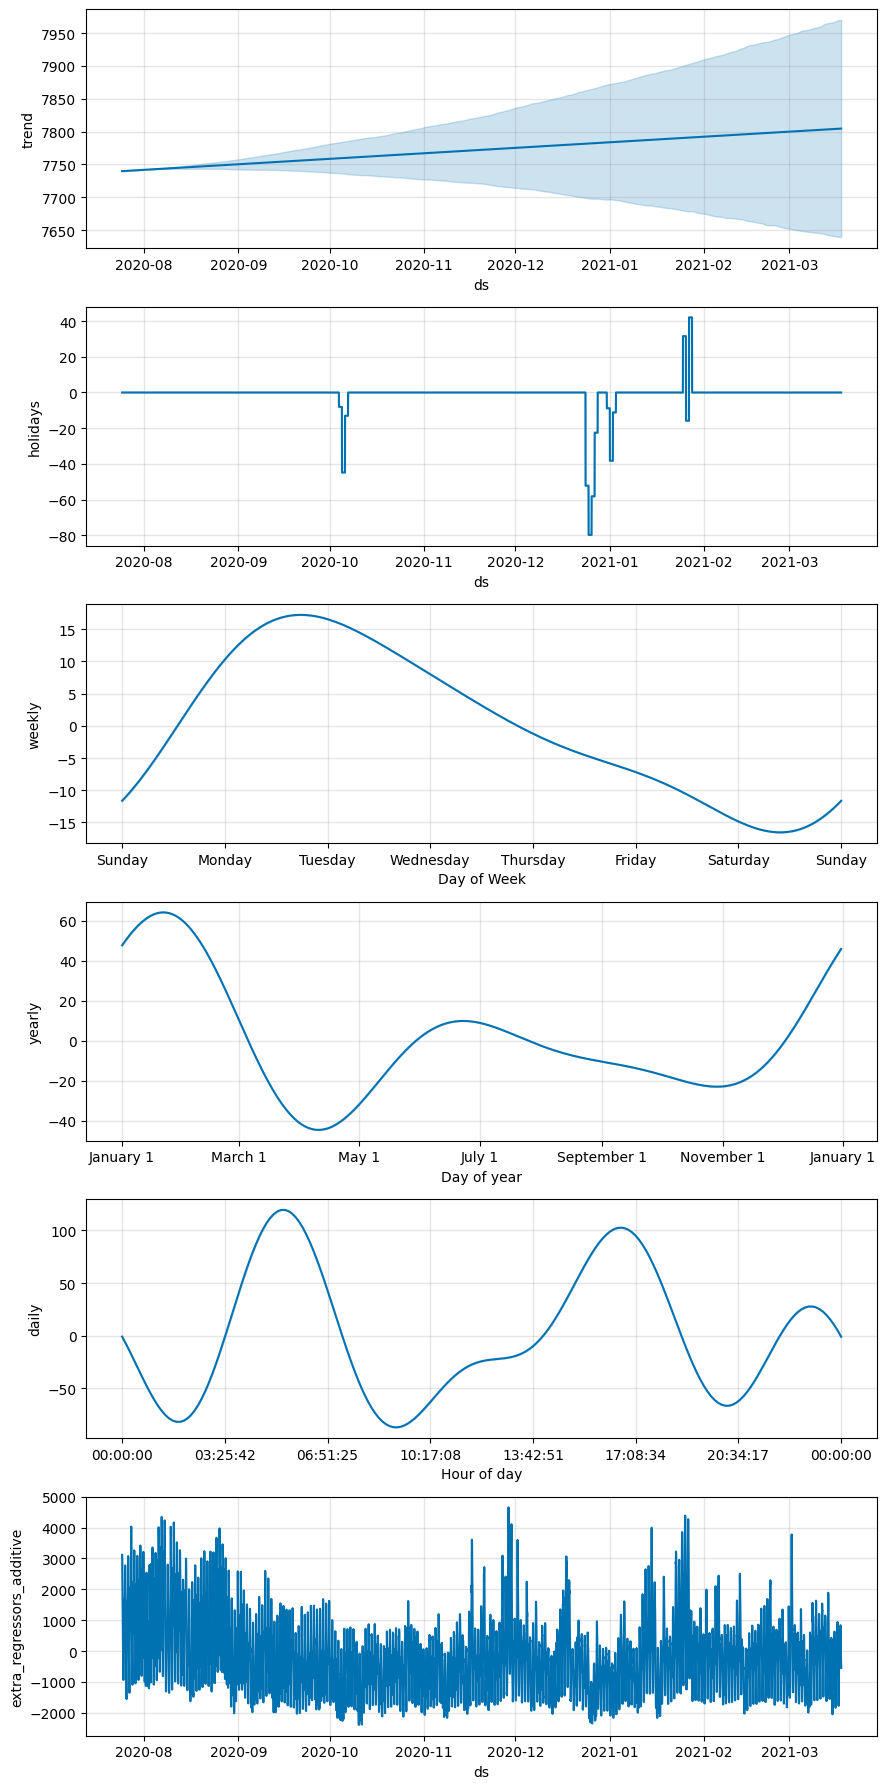
\includegraphics[width=0.95\textwidth, height=10cm]{prophet_component_plot.png}
\caption{Component plots of model Prophet}\label{prophet_component_plot}
\end{figure}

\subsection{Model Forecast}\label{model-forecast}

The Fig \ref{prophet_actual_predict_output} shows the forecast for 17
days for March 2021:

\begin{figure}[H]
\centering
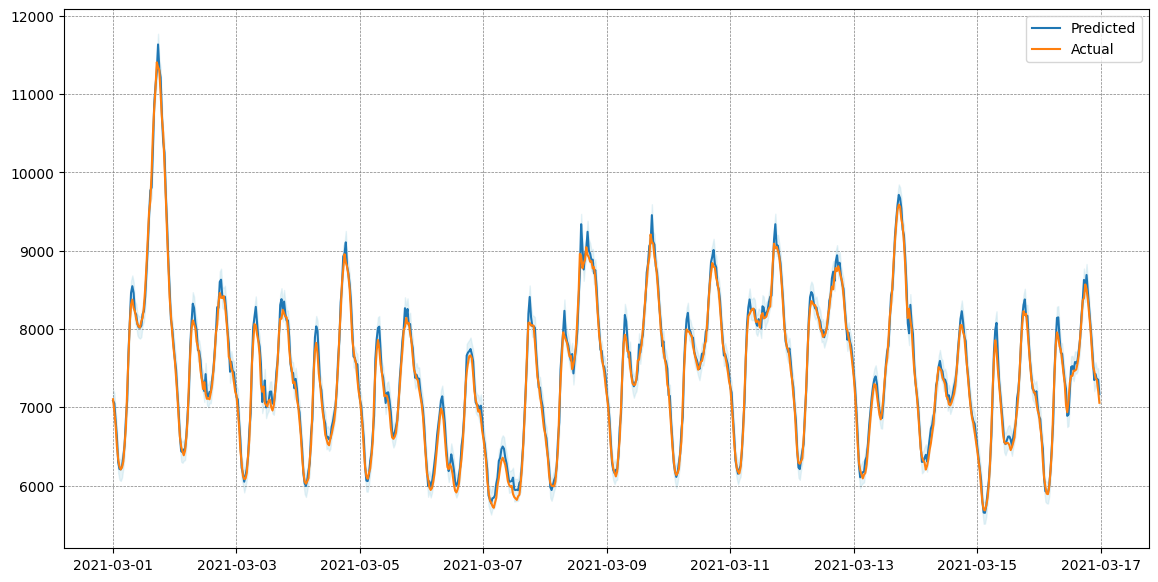
\includegraphics[width=0.95\textwidth, height=5cm]{prophet_actual_predict_output.png}
\caption{Actual vs Predicted demand: Prophet model Prophet}\label{prophet_actual_predict_output}
\end{figure}

\begin{figure}[H]
\centering
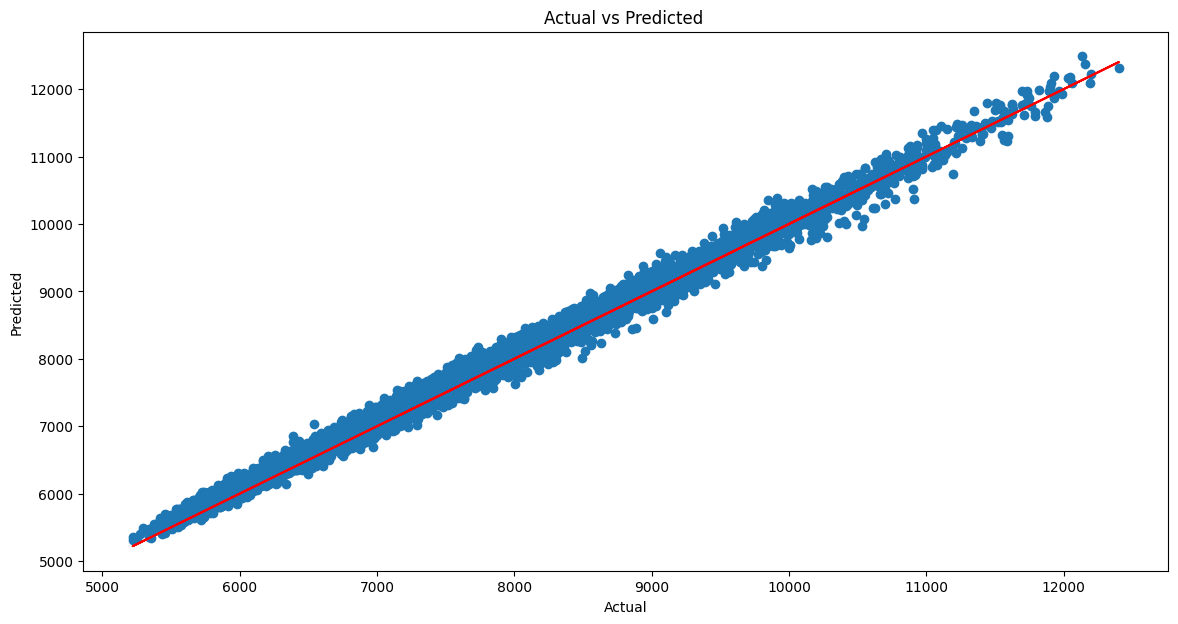
\includegraphics[width=0.95\textwidth, height=5cm]{prophet_actual_predict.png}
\caption{Actual vs Predicted Demaand: Prophet model}\label{prophet_actual}
\end{figure}

\chapter{Model comparison and
Discussion}\label{model-comparison-and-discussion}

XGBoost excels in handling complex non-linear relationships but does not
account for time series components like trends and seasonality. It
requires manual feature engineering to forecast time series data, such
as transforming hours using Cosine and adding a demand lag column to
capture temporal dependencies. However, Facebook Prophet is designed
with time series forecasting in mind. Prophet deploys additive models
that naturally incorporate trends (yearly, monthly, and daily). It is
powerful when handling time series.

Both models are flexible and can process any time interval. XGBoost's
performance is based on the feature engineering approach. For short time
intervals, the features must capture the dynamics of electricity demand
at this granularity. Facebook Prophet automatically detects and captures
patterns in half-hour electricity demand data. Facebook Prophet is more
user-friendly than XGBoost. Its components are understandable, making
understanding the factors influencing the forecast easier. While XGBoost
requires careful feature engineering and parameter tuning, model
interpretation is challenging due to the ensemble nature of the model.

Facebook Prophet is tailored for time series data; It has built-in
mechanisms to capture trends, making it a robust model for electricity
demand forecasting at different intervals. XGBoost has high accuracy in
many domains and is one of the most used models in machine learning
competitions. However, without adequate feature engineering to address
temporal relationships, XGBoost may not perform as effectively as models
designed for time series.

The XGBoost and Facebook Prophet models provided better forecasts than
the model used by AEMO. At first glance, both XGBoost and Facebook
Prophet are outright better models. However, Several factors need to be
considered before making such a claim. Firstly, AEMO's model might be
more general-purpose and work across various regions, time frames, and
applications. The two models we built are tailored to a specific
dataset, time frame, and region, allowing the models to focus on the
unique characteristics of electricity forecast in that context. This
specialisation might explain the better performance in this case.

Hyperparameter tuning is affected by the conditions and adapts to the
exact dataset and timeframe. A small change in a hyperparameter, like
the learning rate or tree depth, can significantly impact results. The
models we built may be finely tuned to capture the patterns in
electricity demand in this context. However, the AEMO model could be
built and tuned to handle various scenarios and time frames.

The models we built focus on short intervals. AEMO model might be
optimised for longer-demand patterns due to operational needs. We
intended to tune for forecasting short-term demand, while the AEMO model
could be tuned for long-term stability. This could explain why our model
performed better when forecasting a short-term interval.

Our models are optimised for a specific time window (30 minutes). Thus,
they are suited to detecting patterns in that period. A more general
model might need help with extreme cases like sharp demand spikes or
sudden peak-hour drops. This could explain why our model performed
better, but this comes at the cost of model forecast period flexibility.
Our model will struggle if used to forecast a long-time horizon compared
to the AEMO model.

The Fig \ref{AEMO_Prophet_XGBoost} shows the comparison of the
forecasted demand among AEMO, XGBoost, and Prophet models. The XGBoost
model follows the actual demand more closely than the Prophet and AEMO
model.

\begin{figure}[H]
\centering
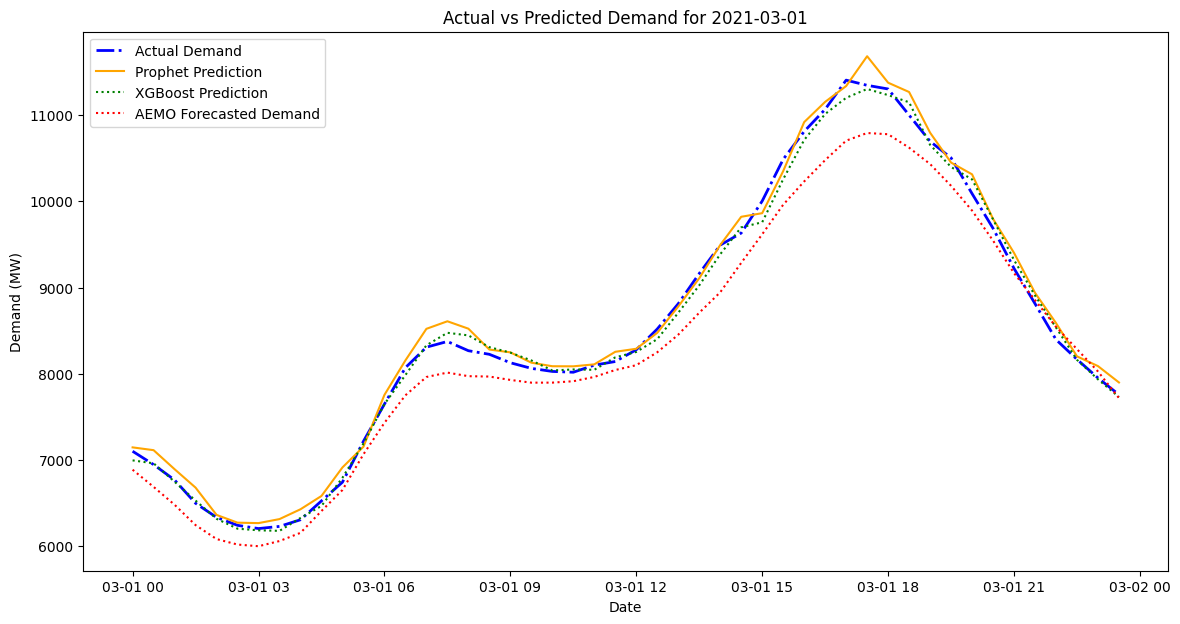
\includegraphics[width=0.95\textwidth, height=5cm]{AEMO_Prophet_XGBoost.png}
\caption{Forecast demand comparison among AEMO, XGBoost and Prophet}\label{AEMO_Prophet_XGBoost}
\end{figure}

\chapter{Conclusion and Future Work}\label{conclusion-and-future-work}

We built, tested, and compared popular machine-learning models --
XGBoost and with an additive model -- Prophet. XGBoost is highly
flexible and known for its high accuracy in many domains, while Facebook
Prophet is a time-series-specific model that excels in capturing trends.
The goal is to see how these different models forecast short-term
electricity demand.

We found that both models performed well with very close results.
Facebook Prophet is easier to use and more efficient when forecasting
electricity demand. It offers a more user-friendly approach because it's
built to handle time series data with clear seasonal patterns. However,
XGBoost can deliver competitive results at the cost of substantial
feature engineering.

We also compared the two models with the AEMO forecast to benchmark our
performance against industry standards, and our models performed better.
However, we do not suggest that our models are superior to AEMO. There
are many valid time horizons for electricity demand forecasting where
the current AEMO model will outperform the models we build. We trained
our model on a specific dataset, while the AEMO model is trained on more
extensive and complex data. The AEMO model is also built to handle
various scenarios. However, our model is built for one specific
scenario.

The results highlight how tailoring a model to a specific forecasting
problem can improve accuracy. By creating particular models, we can
better address electricity demand's short-term, high-frequency nature.
This report emphasises the importance of customisation in forecasting
models. Comparing multi-use multi-timeframe models and single-use case
models is work that needs to be done in the future, along with
incorporating the impact of photovoltaic systems and population and
economic growth.

For future work, we recommend expanding the dataset to include more
features like weather data, economic indicators, and population growth.
This will help the model capture more complex patterns and improve
forecasting accuracy. We also want to recommend the cost-benefit
analysis of implementing the models in real-world scenarios. This will
help stakeholders to choose the best model for their specific needs. We
will also explore popular deep learning models like LSTM and other
pre-trained models like DeepAR for short-term electricity laod
forecasting.

\chapter*{References}\label{references}
\addcontentsline{toc}{chapter}{References}

\bibliographystyle{elsarticle-harv} 
\bibliography{references}

\chapter*{Appendix}\label{appendix}
\addcontentsline{toc}{chapter}{Appendix}

\section*{\texorpdfstring{\textbf{Figures}}{Figures}}\label{figures}
\addcontentsline{toc}{section}{\textbf{Figures}}

\begin{figure}[H]
\centering
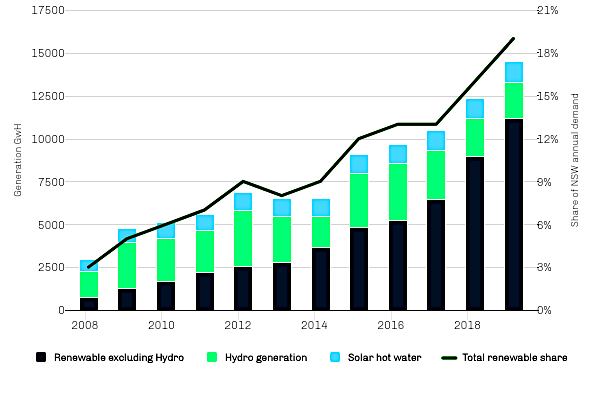
\includegraphics[width=0.5\textwidth,height=7cm]{renewable_fuel_sources_chart.png}
\caption{Renewable fuel sources [Source:
Derived from Department of the Environment and Energy, Australian Energy Statistics, Table O, June 2021]}\label{renewable}
\end{figure}

\section*{\texorpdfstring{\textbf{Codes}}{Codes}}\label{codes}
\addcontentsline{toc}{section}{\textbf{Codes}}

Add you codes here.

\section*{\texorpdfstring{\textbf{Tables}}{Tables}}\label{tables}
\addcontentsline{toc}{section}{\textbf{Tables}}

If you have tables, you can add them here.

Use \url{https://www.tablesgenerator.com/markdown_tables} to create very
simple markdown tables, otherwise use \LaTeX.

\begin{longtable}[]{@{}lcr@{}}
\toprule\noalign{}
Tables & Are & Cool \\
\midrule\noalign{}
\endhead
\bottomrule\noalign{}
\endlastfoot
col 1 is & left-aligned & \$1200 \\
col 2 is & centered & \$12 \\
col 3 is & right-aligned & \$1 \\
\end{longtable}







\end{document}

